\documentclass[10pt]{beamer}
\usetheme{Madrid}
\usecolortheme{seahorse}
\setbeamertemplate{navigation symbols}{}
\usepackage{listings}
\usepackage{xcolor}
\usepackage{amsmath}

\definecolor{codebg}{RGB}{245,245,245}
\definecolor{codekw}{RGB}{0,90,160}
\definecolor{codecomment}{RGB}{90,130,90}
\definecolor{codestr}{RGB}{150,60,30}

\lstset{
  language=Python,
  basicstyle=\ttfamily\scriptsize,
  keywordstyle=\color{codekw}\bfseries,
  commentstyle=\color{codecomment}\itshape,
  stringstyle=\color{codestr},
  backgroundcolor=\color{codebg},
  showstringspaces=false,
  frame=single,
  framerule=0pt,
  xleftmargin=4pt,
  xrightmargin=4pt,
  breaklines=true,
  columns=fullflexible,
  keepspaces=true,
}

\title{Build Two-Way Phase Synchronization}
\subtitle{Code it from the ground up --- the snippets on these slides
ARE the implementation}
\author{Distributed-array phase synchronization project}
\date{}

\begin{document}

\begin{frame}
  \titlepage
\end{frame}

\begin{frame}{How this guide works}
  \begin{itemize}
    \item You are going to write \textbf{one Python file},
      \texttt{build\_twoway.py}, from top to bottom. Each section of
      this deck explains what comes next, then gives you the code to
      type --- \textbf{the snippets, typed in order, are the complete
      file}. Nothing is elided, nothing is toy code.
    \item And the file is not a simplification either: every line is
      \textbf{verbatim from the repository}
      (\texttt{ota\_sync/core.py}, \texttt{sdr.py},
      \texttt{coherent.py}); each section cites its source lines.
      When you finish, you have built the repository's actual two-way
      synchronization --- and running your file reproduces the
      repository's output \textbf{bit for bit} (verified; the check
      is on the last slide).
    \item Requirements: Python with \texttt{torch} and
      \texttt{sionna} $\geq$ 2.0.
    \item What you are building: two stations, each with its own
      drifting clock, exchange pilot waveforms both ways through a
      3GPP multipath channel every 50\,ms; a receiver chain measures
      timing/frequency/phase from raw samples; an extended Kalman
      filter tracks the clock offset; closed-loop corrections hold
      the pair aligned. Final performance, which your file will
      print: coherent gain 99.8\%.
  \end{itemize}
\end{frame}

\begin{frame}{The build order}
  \begin{enumerate}
    \item \textbf{Header} --- imports and the two working dtypes.
    \item \textbf{Small tools} --- \texttt{wrap\_phase}, covariance
      root, device pick.
    \item \textbf{The Oscillator} --- the drifting clock (the enemy).
    \item \textbf{The config} --- every physical assumption in one
      dataclass.
    \item \textbf{The pilot} --- Zadoff--Chu training fields.
    \item \textbf{Hardware imperfections} --- converters, amplifier,
      sample-clock, flicker noise.
    \item \textbf{The radio link} --- Sionna channel + the full
      capture chain.
    \item \textbf{The receiver} --- timing, frequency, phase from raw
      samples; $R$ from physics.
    \item \textbf{The filter} --- the extended Kalman filter.
    \item \textbf{The loop} --- half-difference, branch handling,
      corrections, metrics.
    \item \textbf{Run it} --- and verify against the repository.
  \end{enumerate}
\end{frame}

\begin{frame}{The file header}
  Create \texttt{build\_twoway.py}. First the imports: torch,
  and four Sionna pieces --- the noise block, the channel
  operator, the 3GPP tapped-delay-line model, and two helpers
  that convert a physical channel response into discrete-time
  taps. All numerics run in double precision: phase
  accumulates over millions of samples, and float32 rounding
  would show up as fake oscillator noise.
\end{frame}

\begin{frame}[fragile]{The file header --- type this}
\begin{lstlisting}[basicstyle=\ttfamily\tiny]
"""Two-way over-the-air phase synchronization, built from the ground up.

Every line below is verbatim from ota_sync/ (core.py, sdr.py,
coherent.py) -- only the import header differs, because everything
lives in this one file. Typing this file section by section, as the
coding guide walks it, produces the repository's actual two-way
implementation; running it reproduces the repository's numbers
exactly.
"""

from __future__ import annotations

from dataclasses import dataclass
import math
from typing import Optional

import torch
from sionna.phy import config as sionna_config
from sionna.phy.channel import AWGN, ApplyTimeChannel
from sionna.phy.channel.tr38901 import TDL
from sionna.phy.channel.utils import (
    cir_to_time_channel,
    time_lag_discrete_time_channel,
)

REAL_DTYPE = torch.float64
COMPLEX_DTYPE = torch.complex128
\end{lstlisting}
\end{frame}

\begin{frame}{wrap\_phase}
  A phase is an angle: $370^\circ$ \emph{is} $10^\circ$. Every
  phase subtraction in this program goes through this one-liner,
  or differences near the boundary come out wrong by a full
  turn. It appears on nearly every line that touches a phase;
  when debugging this kind of code, suspect a missing wrap
  first. (Repository: \texttt{core.py:24}.)
\end{frame}

\begin{frame}[fragile]{wrap\_phase --- type this}
\begin{lstlisting}[basicstyle=\ttfamily\tiny]
def wrap_phase(value: torch.Tensor) -> torch.Tensor:
    """Wrap angles in radians to [-pi, pi)."""

    return torch.remainder(value + math.pi, 2.0 * math.pi) - math.pi
\end{lstlisting}
\end{frame}

\begin{frame}{Two small linear-algebra helpers}
  \texttt{\_as\_matrix} is convenience. \texttt{\_covariance\_root}
  matters: to draw correlated noise with covariance $Q$ you need
  a matrix square root of $Q$; an eigendecomposition gives one
  that tolerates positive-\emph{semi}definite $Q$ (a zero
  eigenvalue = a noiseless direction), which a plain Cholesky
  factorization would reject. (\texttt{core.py:50--62}.)
\end{frame}

\begin{frame}[fragile]{Two small linear-algebra helpers --- type this}
\begin{lstlisting}[basicstyle=\ttfamily\tiny]
def _as_matrix(
    value: torch.Tensor | list[list[float]], device: torch.device
) -> torch.Tensor:
    return torch.as_tensor(value, dtype=REAL_DTYPE, device=device)


def _covariance_root(covariance: torch.Tensor) -> torch.Tensor:
    """Return a square root for a positive-semidefinite covariance matrix."""

    eigenvalues, eigenvectors = torch.linalg.eigh(covariance)
    if torch.any(eigenvalues < -1e-12):
        raise ValueError("covariance must be positive semidefinite")
    return eigenvectors @ torch.diag(torch.sqrt(torch.clamp(eigenvalues, min=0.0)))
\end{lstlisting}
\end{frame}

\begin{frame}{resolve\_device}
  Runs on the graphics card when one is available, the
  processor otherwise. (\texttt{core.py:133}.)
\end{frame}

\begin{frame}[fragile]{resolve\_device --- type this}
\begin{lstlisting}[basicstyle=\ttfamily\tiny]
def resolve_device(requested: str) -> torch.device:
    """Resolve ``auto`` to CUDA when available and CPU otherwise."""

    if requested == "auto":
        return torch.device("cuda" if torch.cuda.is_available() else "cpu")
    device = torch.device(requested)
    if device.type == "cuda" and not torch.cuda.is_available():
        raise RuntimeError("CUDA was requested but is not available")
    return device
\end{lstlisting}
\end{frame}

\begin{frame}{The Oscillator -- the enemy}
  The clock model: state $[\theta, \omega]$ (phase, frequency).
  The transition matrix says phase advances by frequency
  $\times$ time. The noise is a \textbf{random walk in both
  components} -- drawn through the covariance root so the two
  components are correctly correlated -- and random walks
  accumulate; they never average away. \texttt{apply\_correction}
  is the actuator the loop will drive; nothing else may touch
  the state. Keep the transition matrix in mind: the Kalman
  filter carries an exact copy of it, so filter and physics
  agree by construction. (\texttt{core.py:175--225}.)
\end{frame}

\begin{frame}[fragile]{The Oscillator -- the enemy --- type this (1/2)}
\begin{lstlisting}[basicstyle=\ttfamily\tiny]
class Oscillator:
    """Random-walk phase and angular-frequency oscillator model."""

    def __init__(
        self,
        initial_phase: float,
        initial_frequency: float,
        sync_interval: float,
        process_covariance: torch.Tensor,
        device: torch.device,
        generator: Optional[torch.Generator] = None,
    ) -> None:
        self.device = device
        self.state = torch.tensor(
            [initial_phase, initial_frequency], dtype=REAL_DTYPE, device=device
        )
        self.transition = torch.tensor(
            [[1.0, sync_interval], [0.0, 1.0]],
            dtype=REAL_DTYPE,
            device=device,
        )
        self.process_covariance = _as_matrix(process_covariance, device)
        if self.process_covariance.shape != (2, 2):
            raise ValueError("process_covariance must have shape [2, 2]")
        self._noise_root = _covariance_root(self.process_covariance)
        
        self._generator = generator
\end{lstlisting}
\end{frame}

\begin{frame}[fragile]{The Oscillator -- the enemy --- type this (2/2)}
\begin{lstlisting}[basicstyle=\ttfamily\tiny]
    @property
    def phase(self) -> torch.Tensor:
        return self.state[0]

    @property
    def frequency(self) -> torch.Tensor:
        return self.state[1]

    def step(self) -> torch.Tensor:
        white_noise = torch.randn(
            2,
            dtype=REAL_DTYPE,
            device=self.device,
            generator=self._generator,
        )
        process_noise = self._noise_root @ white_noise
        self.state = self.transition @ self.state + process_noise
        self.state[0] = wrap_phase(self.state[0])
        return self.state.clone()

    def apply_correction(self, correction: torch.Tensor) -> None:
        self.state = self.state + correction.to(dtype=REAL_DTYPE, device=self.device)
        self.state[0] = wrap_phase(self.state[0])
\end{lstlisting}
\end{frame}

\begin{frame}{SDRSimulationConfig -- every physical assumption}
  One frozen dataclass holds every knob: timing (50\,ms
  intervals, 1\,MHz sampling), the channel (3GPP model ``D'',
  100\,ns delay spread, 915\,MHz), the pilot structure
  ($16\times16$ short, $2047\times2$ long), the oscillator noise
  levels, every hardware impairment, and the loop's actuation
  limits (16-bit phase corrections, one-interval command
  latency, 1\,ms turnaround). Every experiment in the
  repository is a variation of these fields -- never edited
  code. (\texttt{sdr.py:33--94}.)
\end{frame}

\begin{frame}[fragile]{SDRSimulationConfig -- every physical assumption --- type this (1/2)}
\begin{lstlisting}[basicstyle=\ttfamily\tiny]
@dataclass(frozen=True)
class SDRSimulationConfig:
    """Configuration of the sampled-IQ SDR synchronization experiment."""

    sync_interval: float = 0.05
    sample_rate: float = 1e6
    num_iterations: int = 100
    snr_db: float = 20.0
    carrier_frequency_hz: float = 915e6

    tdl_model: str = "D"
    delay_spread_s: float = 100e-9
    maximum_channel_delay_s: float = 3e-6
    channel_speed_mps: float = 0.0

    short_sequence_length: int = 16
    short_repetitions: int = 16
    long_sequence_length: int = 2047
    long_cp_length: int = 128
    long_repetitions: int = 2
    capture_guard_samples: int = 64
    timing_jitter_samples: int = 32

    master_initial_phase: float = 0.0
    master_initial_frequency_hz: float = 0.0
    slave_initial_phase: float = 1.2
    slave_initial_frequency_hz: float = 1500.0
    phase_process_std_rad: float = 0.002
    frequency_process_std_hz: float = 0.1
\end{lstlisting}
\end{frame}

\begin{frame}[fragile]{SDRSimulationConfig -- every physical assumption --- type this (2/2)}
\begin{lstlisting}[basicstyle=\ttfamily\tiny]
    # None derives the sample-clock offset from the carrier offset (shared
    # reference crystal); a number forces a fixed, independent offset.
    sample_clock_offset_ppm: float | None = None
    phase_noise_std_rad: float = 2e-4
    phase_noise_white_pm_std_rad: float = 0.005
    flicker_frequency_std_hz: float = 0.05
    shadowing_std_db: float = 2.0
    shadowing_correlation_s: float = 10.0
    iq_gain_imbalance_db: float = 0.2
    iq_phase_imbalance_deg: float = 1.0
    dc_offset: complex = 0.005 + 0.003j
    adc_bits: int = 12
    dac_bits: int = 12
    tx_amplitude: float = 0.5
    pa_clip_level: float = 0.9
    agc_target_rms: float = 0.25
    detection_threshold: float = 0.25

    phase_correction_bits: int = 16
    frequency_correction_resolution_hz: float = 0.01
    correction_latency_intervals: int = 1
    # Residual TX/RX chain phase asymmetry between the nodes after loopback
    # calibration; it does not cancel in a two-way exchange.
    twoway_chain_asymmetry_deg: float = 0.0
    # Half-duplex (TDD) turnaround inserted between the forward and reverse
    # frames of a two-way exchange. The oscillators keep drifting across the
    # gap; the loop compensates the deterministic part with its own CFO
    # estimate, so the residual penalty is the frequency-estimate error
    # times the gap plus the phase random walk accumulated during it.
    tdd_turnaround_s: float = 1e-3
    seed: int = 0
    device: str = "auto"
\end{lstlisting}
\end{frame}

\begin{frame}{Config validation}
  The dataclass rejects nonsense at construction: negative
  noise levels, a cyclic prefix longer than its sequence, too
  few training repeats. Fail loudly at setup, not silently
  mid-run. The \texttt{sample\_period} property is the only
  derived quantity. (\texttt{sdr.py:96--157}.)
\end{frame}

\begin{frame}[fragile]{Config validation --- type this (1/2)}
\begin{lstlisting}[basicstyle=\ttfamily\tiny]
    def __post_init__(self) -> None:
        if self.sync_interval <= 0.0 or self.sample_rate <= 0.0:
            raise ValueError("sync_interval and sample_rate must be positive")
        if self.num_iterations < 1:
            raise ValueError("num_iterations must be positive")
        if self.carrier_frequency_hz <= 0.0:
            raise ValueError("carrier_frequency_hz must be positive")
        if self.tdl_model not in {
            "A",
            "B",
            "C",
            "D",
            "E",
            "A30",
            "B100",
            "C300",
        }:
            raise ValueError("invalid Sionna TDL model")
        if self.delay_spread_s <= 0.0 or self.maximum_channel_delay_s <= 0.0:
            raise ValueError("channel delays must be positive")
        if self.channel_speed_mps < 0.0:
            raise ValueError("channel_speed_mps cannot be negative")
        if self.short_sequence_length < 2 or self.short_repetitions < 3:
            raise ValueError("the short training field needs at least three repeats")
        if self.long_sequence_length < 3 or self.long_repetitions < 2:
            raise ValueError("the long training field needs at least two repeats")
        if not 0 <= self.long_cp_length < self.long_sequence_length:
            raise ValueError("long_cp_length must be shorter than the long sequence")
        if self.capture_guard_samples < 1 or self.timing_jitter_samples < 0:
            raise ValueError("capture guard must be positive and jitter nonnegative")
\end{lstlisting}
\end{frame}

\begin{frame}[fragile]{Config validation --- type this (2/2)}
\begin{lstlisting}[basicstyle=\ttfamily\tiny]
        if self.phase_process_std_rad < 0.0 or self.frequency_process_std_hz < 0.0:
            raise ValueError("oscillator process deviations cannot be negative")
        if self.phase_noise_std_rad < 0.0:
            raise ValueError("phase_noise_std_rad cannot be negative")
        if self.phase_noise_white_pm_std_rad < 0.0:
            raise ValueError("phase_noise_white_pm_std_rad cannot be negative")
        if self.flicker_frequency_std_hz < 0.0:
            raise ValueError("flicker_frequency_std_hz cannot be negative")
        if self.shadowing_std_db < 0.0:
            raise ValueError("shadowing_std_db cannot be negative")
        if self.shadowing_correlation_s <= 0.0:
            raise ValueError("shadowing_correlation_s must be positive")
        if self.adc_bits < 2 or self.dac_bits < 2:
            raise ValueError("ADC and DAC resolution must be at least two bits")
        if not 0.0 < self.tx_amplitude <= 1.0:
            raise ValueError("tx_amplitude must be in (0, 1]")
        if self.pa_clip_level <= 0.0 or self.agc_target_rms <= 0.0:
            raise ValueError("PA clip level and AGC target must be positive")
        if not 0.0 <= self.detection_threshold <= 1.0:
            raise ValueError("detection_threshold must be in [0, 1]")
        if self.phase_correction_bits < 1:
            raise ValueError("phase_correction_bits must be positive")
        if self.frequency_correction_resolution_hz <= 0.0:
            raise ValueError("frequency correction resolution must be positive")
        if self.correction_latency_intervals < 0:
            raise ValueError("correction_latency_intervals cannot be negative")
        if self.tdd_turnaround_s < 0.0:
            raise ValueError("tdd_turnaround_s cannot be negative")

    @property
    def sample_period(self) -> float:
        return 1.0 / self.sample_rate
\end{lstlisting}
\end{frame}

\begin{frame}{Three small data carriers}
  \texttt{SyncPreamble}: the pilot waveform plus the layout
  facts the receiver needs. \texttt{IQCapture}: what one
  capture returns -- the impaired samples, an impairment-free
  \emph{oracle} copy (ground truth for diagnostics), and the
  end value of the intra-frame oscillator walk, which the loop
  must carry into the clock state. \texttt{SDRMeasurement}:
  what the receiver reports -- detected?, phase, frequency,
  timing, and the detection metric. (\texttt{sdr.py:160--191}.)
\end{frame}

\begin{frame}[fragile]{Three small data carriers --- type this}
\begin{lstlisting}[basicstyle=\ttfamily\tiny]
@dataclass(frozen=True)
class SyncPreamble:
    waveform: torch.Tensor
    short_sequence: torch.Tensor
    long_sequence: torch.Tensor
    short_length: int
    long_block_length: int

    @property
    def length(self) -> int:
        return self.waveform.numel()


@dataclass(frozen=True)
class IQCapture:
    samples: torch.Tensor
    oracle_samples: torch.Tensor
    lo_walk_end: torch.Tensor
    inserted_start: int
    expected_arrival: int
    agc_gain: float
    clip_rate: float


@dataclass(frozen=True)
class SDRMeasurement:
    detected: bool
    phase: torch.Tensor
    frequency: torch.Tensor
    timing_index: int
    detection_metric: float
\end{lstlisting}
\end{frame}

\begin{frame}{The pilot: Zadoff--Chu training fields}
  Constant-amplitude chirps with a single-spike
  autocorrelation -- the same family LTE and 5G use. The
  preamble is $16\times16$ short repeats (for coarse timing and
  frequency) then $2047\times2$ long sequences with a cyclic
  prefix (for fine frequency and phase). Why 2047: the
  frequency-estimate error times the 50\,ms interval is phase
  drift the loop must ride out, and it must stay far inside
  the $\pm\pi/2$ branch boundary you will meet later.
  (\texttt{sdr.py:253--288}.)
\end{frame}

\begin{frame}[fragile]{The pilot: Zadoff--Chu training fields --- type this (1/2)}
\begin{lstlisting}[basicstyle=\ttfamily\tiny]
def _zadoff_chu(length: int, root: int, device: torch.device) -> torch.Tensor:
    if math.gcd(length, root) != 1:
        raise ValueError("Zadoff-Chu root and length must be coprime")
    n = torch.arange(length, dtype=REAL_DTYPE, device=device)
    if length % 2:
        phase = -math.pi * root * n * (n + 1.0) / length
    else:
        phase = -math.pi * root * n.square() / length
    return torch.exp(1j * phase).to(COMPLEX_DTYPE)


def make_sync_preamble(
    settings: SDRSimulationConfig, device: torch.device
) -> SyncPreamble:
    """Construct short and long SDR synchronization training fields."""

    short = _zadoff_chu(settings.short_sequence_length, 1, device)
    long_root = 25
    while math.gcd(settings.long_sequence_length, long_root) != 1:
        long_root += 1
    long = _zadoff_chu(settings.long_sequence_length, long_root, device)
    short_field = short.repeat(settings.short_repetitions)
    cyclic_prefix = (
        long[-settings.long_cp_length :] if settings.long_cp_length else long[:0]
    )
    long_block = torch.cat((cyclic_prefix, long))
    long_field = long_block.repeat(settings.long_repetitions)
    waveform = torch.cat((short_field, long_field))
    return SyncPreamble(
        waveform=waveform,
\end{lstlisting}
\end{frame}

\begin{frame}[fragile]{The pilot: Zadoff--Chu training fields --- type this (2/2)}
\begin{lstlisting}[basicstyle=\ttfamily\scriptsize]
        short_sequence=short,
        long_sequence=long,
        short_length=short_field.numel(),
        long_block_length=long_block.numel(),
    )
\end{lstlisting}
\end{frame}

\begin{frame}{Converter and clock imperfections}
  \texttt{\_quantize\_iq}: a $b$-bit converter -- clip to full
  scale, round to the grid, report the clip rate.
  \texttt{\_soft\_limit}: the power amplifier's gentle
  saturation. \texttt{\_resample\_clock\_offset}: the receiver's
  sample clock runs at a slightly different rate than the
  transmitter's, so the samples are linearly re-interpolated at
  the offset rate plus a fractional delay.
  (\texttt{sdr.py:290--325}.)
\end{frame}

\begin{frame}[fragile]{Converter and clock imperfections --- type this (1/2)}
\begin{lstlisting}[basicstyle=\ttfamily\tiny]
def _quantize_iq(samples: torch.Tensor, bits: int) -> tuple[torch.Tensor, float]:
    limit = float(2 ** (bits - 1) - 1)
    real = samples.real
    imag = samples.imag
    clipped = (real.abs() > 1.0) | (imag.abs() > 1.0)
    real = torch.round(torch.clamp(real, -1.0, 1.0) * limit) / limit
    imag = torch.round(torch.clamp(imag, -1.0, 1.0) * limit) / limit
    return torch.complex(real, imag), torch.mean(clipped.to(REAL_DTYPE)).item()


def _soft_limit(samples: torch.Tensor, limit: float) -> torch.Tensor:
    magnitude = torch.abs(samples)
    scale = torch.clamp(limit / torch.clamp(magnitude, min=1e-15), max=1.0)
    return samples * scale


def _resample_clock_offset(
    samples: torch.Tensor, ppm: float, delay_samples: float = 0.0
) -> torch.Tensor:
    """Linearly resample IQ at a receiver clock offset and fractional delay."""
\end{lstlisting}
\end{frame}

\begin{frame}[fragile]{Converter and clock imperfections --- type this (2/2)}
\begin{lstlisting}[basicstyle=\ttfamily\tiny]
    if ppm == 0.0 and delay_samples == 0.0:
        return samples
    ratio = 1.0 + ppm * 1e-6
    output_index = torch.arange(
        samples.numel(), dtype=REAL_DTYPE, device=samples.device
    )
    source = output_index / ratio - delay_samples
    lower = torch.floor(source).to(torch.int64)
    upper = lower + 1
    valid = (lower >= 0) & (upper < samples.numel())
    lower = torch.clamp(lower, 0, samples.numel() - 1)
    upper = torch.clamp(upper, 0, samples.numel() - 1)
    fraction = source - lower.to(REAL_DTYPE)
    output = samples[lower] * (1.0 - fraction) + samples[upper] * fraction
    return torch.where(valid, output, torch.zeros_like(output))
\end{lstlisting}
\end{frame}

\begin{frame}{Flicker frequency noise}
  Real oscillators have $1/f$ frequency noise on top of the
  white walks. The standard time-domain surrogate: a bank of
  four first-order decaying processes with log-spaced time
  constants, summed. The class also exposes its per-interval
  \texttt{innovation\_variance} -- the loop adds it to the
  filter's process noise, so the filter knows about this noise
  source too. (\texttt{sdr.py:328--391}.)
\end{frame}

\begin{frame}[fragile]{Flicker frequency noise --- type this (1/2)}
\begin{lstlisting}[basicstyle=\ttfamily\tiny]
class _FlickerFrequencyNoise:
    """Approximate flicker FM with a bank of first-order Gauss-Markov processes.

    A sum of AR(1) components with log-spaced correlation times approximates a
    1/f frequency-noise spectrum across the timescales the simulation spans,
    which is the standard time-domain surrogate for flicker FM.
    """

    def __init__(
        self,
        std_hz: float,
        interval_s: float,
        horizon_s: float,
        device: torch.device,
        generator: torch.Generator,
        components: int = 4,
    ) -> None:
        self.device = device
        self.generator = generator
        self.enabled = std_hz > 0.0
        if not self.enabled:
            self.innovation_variance = 0.0
            return
        shortest = 2.0 * interval_s
        longest = max(horizon_s, 4.0 * interval_s)
        exponents = torch.linspace(
            math.log10(shortest),
            math.log10(longest),
            components,
            dtype=REAL_DTYPE,
\end{lstlisting}
\end{frame}

\begin{frame}[fragile]{Flicker frequency noise --- type this (2/2)}
\begin{lstlisting}[basicstyle=\ttfamily\tiny]
            device=device,
        )
        correlation_times = torch.pow(
            torch.tensor(10.0, dtype=REAL_DTYPE, device=device), exponents
        )
        self.rho = torch.exp(-interval_s / correlation_times)
        component_std = 2.0 * math.pi * std_hz / math.sqrt(components)
        self.sigma = torch.full(
            (components,), component_std, dtype=REAL_DTYPE, device=device
        )
        self.state = self.sigma * torch.randn(
            components, dtype=REAL_DTYPE, device=device, generator=generator
        )
        self.innovation_variance = float(
            torch.sum(2.0 * self.sigma.square() * (1.0 - self.rho)).item()
        )

    def step(self) -> torch.Tensor:
        """Advance one interval; return the flicker frequency offset in rad/s."""

        if not self.enabled:
            return torch.zeros((), dtype=REAL_DTYPE, device=self.device)
        innovation = (
            torch.randn(
                self.sigma.numel(),
                dtype=REAL_DTYPE,
                device=self.device,
                generator=self.generator,
            )
            * self.sigma
            * torch.sqrt(1.0 - self.rho.square())
        )
        self.state = self.rho * self.state + innovation
        return torch.sum(self.state)
\end{lstlisting}
\end{frame}

\begin{frame}{SDRRadioLink: the channel}
  The propagation channel is Sionna's 3GPP tapped-delay-line,
  converted to a 16-tap discrete-time filter, one realization
  per sync interval. \textbf{\texttt{mirror\_of} is reciprocity
  in one argument}: the reverse link of a two-way pair shares
  the forward link's taps and shadowing -- the physical fact
  the entire method stands on. The noise floor is fixed at the
  nominal channel gain, so fading changes the actual
  signal-to-noise ratio, as in the field.
  (\texttt{sdr.py:394--473}.)
\end{frame}

\begin{frame}[fragile]{SDRRadioLink: the channel --- type this (1/3)}
\begin{lstlisting}[basicstyle=\ttfamily\tiny]
class SDRRadioLink:
    """Sampled-IQ transmit/channel/receive chain using Sionna TDL and AWGN."""

    def __init__(
        self,
        settings: SDRSimulationConfig,
        preamble: SyncPreamble,
        device: torch.device,
        generator: torch.Generator,
        mirror_of: "SDRRadioLink | None" = None,
        captures_per_interval: int = 1,
    ) -> None:
        self.settings = settings
        self.preamble = preamble
        self.device = device
        self.generator = generator
        self.captures_per_interval = captures_per_interval
        # A mirrored link models the reverse direction of a reciprocal
        # channel: it shares the taps and shadowing of the forward link (which
        # must capture first each interval) while keeping its own receiver
        # state (timing carry, noise floor).
        self._mirror = mirror_of
        self._last_shadow_amplitude = 1.0
        self.input_length = (
            preamble.length
            + 2 * settings.capture_guard_samples
            + settings.timing_jitter_samples
        )
        self.l_min, self.l_max = time_lag_discrete_time_channel(
            settings.sample_rate, settings.maximum_channel_delay_s
\end{lstlisting}
\end{frame}

\begin{frame}[fragile]{SDRRadioLink: the channel --- type this (2/3)}
\begin{lstlisting}[basicstyle=\ttfamily\tiny]
        )
        self.l_tot = self.l_max - self.l_min + 1
        self.interval_samples = int(
            round(settings.sync_interval * settings.sample_rate)
        )
        # Receiver clock error accumulated since the capture window was last
        # re-centered, in samples.
        self._timing_carry = 0.0
        # Thermal noise floor, fixed after the first frame at the nominal
        # (unshadowed) channel gain so fading changes the actual SNR.
        self._noise_power: torch.Tensor | None = None
        self._shadow_rho = math.exp(
            -settings.sync_interval / settings.shadowing_correlation_s
        )
        self._shadow_db = settings.shadowing_std_db * torch.randn(
            (), dtype=REAL_DTYPE, device=device, generator=generator
        )

        if mirror_of is not None:
            self.channel_taps = mirror_of.channel_taps
        else:
            self.tdl = TDL(
                model=settings.tdl_model,
                delay_spread=settings.delay_spread_s,
                carrier_frequency=settings.carrier_frequency_hz,
                min_speed=settings.channel_speed_mps,
                max_speed=settings.channel_speed_mps,
                precision="double",
                device=str(device),
            )
\end{lstlisting}
\end{frame}

\begin{frame}[fragile]{SDRRadioLink: the channel --- type this (3/3)}
\begin{lstlisting}[basicstyle=\ttfamily\tiny]
            coefficients, delays = self.tdl(
                batch_size=1,
                num_time_steps=settings.num_iterations,
                sampling_frequency=1.0 / settings.sync_interval,
            )
            self.channel_taps = cir_to_time_channel(
                settings.sample_rate,
                coefficients,
                delays,
                self.l_min,
                self.l_max,
                normalize=True,
            )
        self._apply_channel = ApplyTimeChannel(
            num_time_samples=self.input_length,
            l_tot=self.l_tot,
            precision="double",
            device=str(device),
        )
        self._awgn = AWGN(precision="double", device=str(device))
\end{lstlisting}
\end{frame}

\begin{frame}{Link helpers: jitter and shadowing}
  \texttt{\_random\_start}: the capture window lands with
  random timing jitter. \texttt{\_channel\_for\_frame}: this
  interval's taps, shaped for Sionna's channel operator.
  \texttt{\_step\_shadowing}: slow log-normal fading as a
  correlated process -- and the mirrored link reuses the
  forward link's draw (reciprocity again).
  (\texttt{sdr.py:475--508}.)
\end{frame}

\begin{frame}[fragile]{Link helpers: jitter and shadowing --- type this}
\begin{lstlisting}[basicstyle=\ttfamily\tiny]
    def _random_start(self) -> int:
        jitter = torch.randint(
            self.settings.timing_jitter_samples + 1,
            (),
            device=self.device,
            generator=self.generator,
        ).item()
        return self.settings.capture_guard_samples + jitter

    def _channel_for_frame(self, iteration: int) -> torch.Tensor:
        output_length = self.input_length + self.l_tot - 1
        taps = self.channel_taps[..., iteration, :].unsqueeze(-2)
        return taps.expand(*taps.shape[:-2], output_length, self.l_tot)

    def _step_shadowing(self) -> float:
        """Advance the temporally correlated log-normal shadowing process."""

        if self._mirror is not None:
            # Reciprocity: reuse the forward link's shadowing for this frame.
            return self._mirror._last_shadow_amplitude
        if self.settings.shadowing_std_db <= 0.0:
            self._last_shadow_amplitude = 1.0
            return 1.0
        innovation = torch.randn(
            (), dtype=REAL_DTYPE, device=self.device, generator=self.generator
        )
        self._shadow_db = (
            self._shadow_rho * self._shadow_db
            + math.sqrt(1.0 - self._shadow_rho**2)
            * self.settings.shadowing_std_db
            * innovation
        )
        self._last_shadow_amplitude = float(10.0 ** (self._shadow_db.item() / 20.0))
        return self._last_shadow_amplitude
\end{lstlisting}
\end{frame}

\begin{frame}{capture(), transmit side}
  One direction of one exchange, in physical order: the
  receiver's sample-clock error moves the arrival window
  (whole samples step it; the sub-sample residue stays as a
  fractional delay); the transmitter imprints \emph{its}
  oscillator on the waveform; the power amplifier soft-clips;
  the DAC quantizes; Sionna's channel convolves; shadowing
  scales. (\texttt{sdr.py:510--544}.)
\end{frame}

\begin{frame}[fragile]{capture(), transmit side --- type this (1/2)}
\begin{lstlisting}[basicstyle=\ttfamily\tiny]
    def capture(
        self, master: Oscillator, slave: Oscillator, iteration: int, sfo_ppm: float
    ) -> IQCapture:
        settings = self.settings
        # Clock error accumulates between frames. The receiver re-centers its
        # window on each detection, so whole-sample drift steps the insertion
        # point while the sub-sample residual remains as a fractional delay.
        self._timing_carry += (
            sfo_ppm * 1e-6 * self.interval_samples / self.captures_per_interval
        )
        drift_step = int(round(self._timing_carry))
        self._timing_carry -= drift_step
        fractional_delay = self._timing_carry
        start = self._random_start() + drift_step
        start = min(max(start, 0), self.input_length - self.preamble.length)
        center = start + (self.preamble.length - 1) / 2.0
        sample_index = torch.arange(
            self.input_length, dtype=REAL_DTYPE, device=self.device
        )
        time = (sample_index - center) * settings.sample_period

        frame = torch.zeros(self.input_length, dtype=COMPLEX_DTYPE, device=self.device)
        frame[start : start + self.preamble.length] = (
            settings.tx_amplitude * self.preamble.waveform
        )
        master_carrier = torch.exp(1j * (master.phase + master.frequency * time))
        tx = _soft_limit(frame * master_carrier, settings.pa_clip_level)
        tx, _ = _quantize_iq(tx, settings.dac_bits)
\end{lstlisting}
\end{frame}

\begin{frame}[fragile]{capture(), transmit side --- type this (2/2)}
\begin{lstlisting}[basicstyle=\ttfamily\scriptsize]
        channel_input = tx.reshape(1, 1, 1, -1)
        clean = self._apply_channel(
            channel_input, self._channel_for_frame(iteration)
        ).reshape(-1)
        shadow_amplitude = self._step_shadowing()
        clean = clean * shadow_amplitude
\end{lstlisting}
\end{frame}

\begin{frame}{capture(), receive side}
  Thermal noise at the fixed floor; sample-clock resampling;
  down-conversion with the \emph{receiver's} oscillator (what
  remains is the clock difference plus the channel); the
  oscillator's own random walk \emph{during} the frame -- whose
  end value is returned so the loop keeps the noise continuous
  across frames; white phase jitter; IQ imbalance; automatic
  gain control; DC offset; 12-bit quantization. Every phase
  error the filter must fight is created here, physically.
  (\texttt{sdr.py:545--618}.)
\end{frame}

\begin{frame}[fragile]{capture(), receive side --- type this (1/3)}
\begin{lstlisting}[basicstyle=\ttfamily\tiny]
        active_start = max(0, start - self.l_min)
        active_stop = min(clean.numel(), active_start + self.preamble.length)
        if self._noise_power is None:
            nominal_power = torch.mean(
                torch.abs(clean[active_start:active_stop] / shadow_amplitude).square()
            )
            self._noise_power = nominal_power / (10.0 ** (settings.snr_db / 10.0))
        received = self._awgn(clean, self._noise_power)

        received = _resample_clock_offset(received, sfo_ppm, fractional_delay)
        # The oracle path shares the frame, channel realization, shadowing,
        # deterministic transmit hardware, and sample-clock timing, but carries
        # no stochastic noise or receiver impairments. It defines the
        # ground-truth observable.
        oracle = _resample_clock_offset(clean, sfo_ppm, fractional_delay)
        output_index = torch.arange(
            received.numel(), dtype=REAL_DTYPE, device=self.device
        )
        physical_index = output_index / (1.0 + sfo_ppm * 1e-6) + self.l_min
        receive_time = (physical_index - center) * settings.sample_period
        slave_carrier = torch.exp(-1j * (slave.phase + slave.frequency * receive_time))
        received = received * slave_carrier
        oracle = oracle * slave_carrier
\end{lstlisting}
\end{frame}

\begin{frame}[fragile]{capture(), receive side --- type this (2/3)}
\begin{lstlisting}[basicstyle=\ttfamily\tiny]
        lo_walk_end = torch.zeros((), dtype=REAL_DTYPE, device=self.device)
        if settings.phase_noise_std_rad > 0.0:
            phase_noise = torch.cumsum(
                torch.randn(
                    received.numel(),
                    dtype=REAL_DTYPE,
                    device=self.device,
                    generator=self.generator,
                )
                * settings.phase_noise_std_rad,
                dim=0,
            )
            received = received * torch.exp(1j * phase_noise)
            # End value of the intra-frame walk; the caller carries it into
            # the oscillator state so the LO noise is one continuous process.
            lo_walk_end = phase_noise[-1]

        if settings.phase_noise_white_pm_std_rad > 0.0:
            jitter = (
                torch.randn(
                    received.numel(),
                    dtype=REAL_DTYPE,
                    device=self.device,
                    generator=self.generator,
                )
                * settings.phase_noise_white_pm_std_rad
            )
            received = received * torch.exp(1j * jitter)
\end{lstlisting}
\end{frame}

\begin{frame}[fragile]{capture(), receive side --- type this (3/3)}
\begin{lstlisting}[basicstyle=\ttfamily\tiny]
        gain_ratio = 10.0 ** (settings.iq_gain_imbalance_db / 40.0)
        phase_skew = math.radians(settings.iq_phase_imbalance_deg)
        in_phase = received.real * gain_ratio
        quadrature = received.imag / gain_ratio
        quadrature = quadrature * math.cos(phase_skew) + in_phase * math.sin(phase_skew)
        received = torch.complex(in_phase, quadrature)

        rms = torch.sqrt(torch.mean(torch.abs(received).square()))
        agc_gain = torch.clamp(settings.agc_target_rms / rms, 0.01, 1000.0)
        received = received * agc_gain + settings.dc_offset
        received, clip_rate = _quantize_iq(received, settings.adc_bits)

        return IQCapture(
            samples=received,
            oracle_samples=oracle,
            lo_walk_end=lo_walk_end,
            inserted_start=start,
            expected_arrival=start - self.l_min,
            agc_gain=agc_gain.item(),
            clip_rate=clip_rate,
        )
\end{lstlisting}
\end{frame}

\begin{frame}{The receiver, stage 1: coarse timing and frequency}
  The receiver knows neither when the pilot arrives nor the
  frequency offset. Correlating the signal with itself 16
  samples later solves both at once: when the repeating short
  field fills the window, consecutive repeats match -- the
  normalized magnitude peaks (timing), and the angle between
  repeats is the offset accumulated over 16 samples
  (frequency, unambiguous to $\pm f_s/32 = \pm31$\,kHz).
  (\texttt{sdr.py:621--659}.)
\end{frame}

\begin{frame}[fragile]{The receiver, stage 1: coarse timing and frequency --- type this (1/2)}
\begin{lstlisting}[basicstyle=\ttfamily\tiny]
def _sliding_sum(values: torch.Tensor, width: int) -> torch.Tensor:
    cumulative = torch.cat(
        (
            torch.zeros(1, dtype=values.dtype, device=values.device),
            torch.cumsum(values, dim=0),
        )
    )
    return cumulative[width:] - cumulative[:-width]


class SDRSynchronizer:
    """Packet detector and two-stage carrier synchronizer."""

    def __init__(
        self,
        settings: SDRSimulationConfig,
        preamble: SyncPreamble,
    ) -> None:
        self.settings = settings
        self.preamble = preamble
\end{lstlisting}
\end{frame}

\begin{frame}[fragile]{The receiver, stage 1: coarse timing and frequency --- type this (2/2)}
\begin{lstlisting}[basicstyle=\ttfamily\tiny]
    def _coarse_timing_and_frequency(
        self, samples: torch.Tensor
    ) -> tuple[int, torch.Tensor]:
        lag = self.settings.short_sequence_length
        width = self.preamble.short_length - lag
        product = torch.conj(samples[:-lag]) * samples[lag:]
        first_power = torch.abs(samples[:-lag]).square()
        second_power = torch.abs(samples[lag:]).square()
        correlation = _sliding_sum(product, width)
        normalization = torch.sqrt(
            _sliding_sum(first_power, width) * _sliding_sum(second_power, width)
        ).clamp_min(1e-15)
        metric = torch.abs(correlation) / normalization
        coarse_start = int(torch.argmax(metric).item())
        frequency = torch.angle(correlation[coarse_start]) / (
            lag * self.settings.sample_period
        )
        return coarse_start, frequency
\end{lstlisting}
\end{frame}

\begin{frame}{The receiver, stages 2--3: detect, refine, read the phase}
  Stage 2: after coarse derotation, the \emph{whole} preamble
  is matched against every window; the normalized peak gives
  precise timing, and its height is the detection metric --
  below the 0.25 threshold the capture is declared failed and
  the loop must coast. Stage 3: the two long fields are
  identical and 2175 samples apart; the angle between them
  refines the frequency to $\sim$0.1\,Hz. Finally, derotate
  with the refined frequency (indices centered so the phase is
  referenced to frame \emph{center}) and matched-filter the
  long fields: the correlation angle is the carrier phase --
  clock offset \textbf{plus the channel's phase}. Separating
  those two is the loop's job. (\texttt{sdr.py:661--754}.)
\end{frame}

\begin{frame}[fragile]{The receiver, stages 2--3: detect, refine, read the phase --- type this (1/3)}
\begin{lstlisting}[basicstyle=\ttfamily\tiny]
    def estimate(self, samples: torch.Tensor) -> SDRMeasurement:
        samples = samples - torch.mean(samples)
        coarse_start, coarse_frequency = self._coarse_timing_and_frequency(samples)

        sample_index = torch.arange(
            samples.numel(), dtype=REAL_DTYPE, device=samples.device
        )
        coarse_corrected = samples * torch.exp(
            -1j
            * coarse_frequency
            * (sample_index - coarse_start)
            * self.settings.sample_period
        )

        if coarse_corrected.numel() < self.preamble.length:
            return SDRMeasurement(
                False,
                torch.zeros((), dtype=REAL_DTYPE, device=samples.device),
                coarse_frequency,
                coarse_start,
                0.0,
            )
        windows = coarse_corrected.unfold(0, self.preamble.length, 1)
        correlations = torch.sum(windows * torch.conj(self.preamble.waveform), dim=-1)
        window_energy = torch.sum(torch.abs(windows).square(), dim=-1)
        reference_energy = torch.sum(torch.abs(self.preamble.waveform).square())
        normalized = torch.abs(correlations) / torch.sqrt(
            (window_energy * reference_energy).clamp_min(1e-15)
        )
        timing = int(torch.argmax(normalized).item())
\end{lstlisting}
\end{frame}

\begin{frame}[fragile]{The receiver, stages 2--3: detect, refine, read the phase --- type this (2/3)}
\begin{lstlisting}[basicstyle=\ttfamily\tiny]
        detection_metric = normalized[timing].item()

        short = samples[timing : timing + self.preamble.short_length]
        lag = self.settings.short_sequence_length
        short_correlation = torch.sum(torch.conj(short[:-lag]) * short[lag:])
        coarse_frequency = torch.angle(short_correlation) / (
            lag * self.settings.sample_period
        )

        segment = samples[timing : timing + self.preamble.length]
        relative_index = torch.arange(
            segment.numel(), dtype=REAL_DTYPE, device=samples.device
        )
        coarse_segment = segment * torch.exp(
            -1j * coarse_frequency * relative_index * self.settings.sample_period
        )

        first_start = self.preamble.short_length + self.settings.long_cp_length
        last_start = (
            self.preamble.short_length
            + (self.settings.long_repetitions - 1) * self.preamble.long_block_length
            + self.settings.long_cp_length
        )
        first_long = coarse_segment[
            first_start : first_start + self.settings.long_sequence_length
        ]
        last_long = coarse_segment[
            last_start : last_start + self.settings.long_sequence_length
        ]
        separation = (
\end{lstlisting}
\end{frame}

\begin{frame}[fragile]{The receiver, stages 2--3: detect, refine, read the phase --- type this (3/3)}
\begin{lstlisting}[basicstyle=\ttfamily\tiny]
            self.settings.long_repetitions - 1
        ) * self.preamble.long_block_length
        fine_correlation = torch.sum(torch.conj(first_long) * last_long)
        fine_frequency = torch.angle(fine_correlation) / (
            separation * self.settings.sample_period
        )
        frequency = coarse_frequency + fine_frequency

        centered_index = relative_index - (self.preamble.length - 1) / 2.0
        corrected = segment * torch.exp(
            -1j * frequency * centered_index * self.settings.sample_period
        )
        phase_correlation = torch.zeros((), dtype=COMPLEX_DTYPE, device=samples.device)
        for repeat in range(self.settings.long_repetitions):
            sequence_start = (
                self.preamble.short_length
                + repeat * self.preamble.long_block_length
                + self.settings.long_cp_length
            )
            sequence = corrected[
                sequence_start : sequence_start + self.settings.long_sequence_length
            ]
            phase_correlation += torch.sum(
                torch.conj(self.preamble.long_sequence) * sequence
            )
        phase = torch.angle(phase_correlation)
        detected = detection_metric >= self.settings.detection_threshold
        return SDRMeasurement(
            detected=detected,
            phase=phase,
            frequency=frequency,
            timing_index=timing,
            detection_metric=detection_metric,
        )
\end{lstlisting}
\end{frame}

\begin{frame}{R from physics, and quantized corrections}
  The filter's measurement covariance is \textbf{derived, not
  tuned}: the textbook estimation bound for a pilot of this
  length and signal-to-noise ratio, plus the phase noise the
  oscillator smears across the frame, plus per-sample jitter.
  This is why no gain is hand-tuned anywhere.
  \texttt{\_quantize\_correction} snaps commands to what
  hardware can apply: 16-bit phase steps, 0.01\,Hz frequency
  steps. (\texttt{sdr.py:757--815}.)
\end{frame}

\begin{frame}[fragile]{R from physics, and quantized corrections --- type this (1/2)}
\begin{lstlisting}[basicstyle=\ttfamily\tiny]
def _measurement_covariance(
    settings: SDRSimulationConfig, preamble: SyncPreamble, device: torch.device
) -> torch.Tensor:
    snr = 10.0 ** (settings.snr_db / 10.0)
    phase_variance = 1.0 / (
        2.0 * snr * settings.long_sequence_length * settings.long_repetitions
    )
    separation_time = (
        (settings.long_repetitions - 1)
        * preamble.long_block_length
        * settings.sample_period
    )
    frequency_variance = 1.0 / (
        snr * settings.long_sequence_length * separation_time**2
    )
    # The receiver LO phase noise accumulates as a random walk across the
    # frame and usually dominates the AWGN Cramer-Rao bound. The phase
    # estimate averages the walk over the long training fields, and the fine
    # CFO estimate differences the walk between the two fields.
    long_field_offset = preamble.short_length + settings.long_cp_length
    long_field_span = preamble.length - long_field_offset
    phase_noise_variance = settings.phase_noise_std_rad**2
    phase_variance += phase_noise_variance * (
        long_field_offset + long_field_span / 3.0
    )
    separation_samples = (
        settings.long_repetitions - 1
    ) * preamble.long_block_length
    frequency_variance += (
        phase_noise_variance * separation_samples / separation_time**2
\end{lstlisting}
\end{frame}

\begin{frame}[fragile]{R from physics, and quantized corrections --- type this (2/2)}
\begin{lstlisting}[basicstyle=\ttfamily\tiny]
    )
    # White PM adds an independent phase jitter per sample; it averages down
    # over the long training fields but still belongs in the noise budget.
    white_pm_variance = settings.phase_noise_white_pm_std_rad**2
    total_long_samples = settings.long_sequence_length * settings.long_repetitions
    phase_variance += white_pm_variance / total_long_samples
    frequency_variance += 2.0 * white_pm_variance / (
        settings.long_sequence_length * separation_time**2
    )
    return torch.diag(
        torch.tensor(
            [phase_variance, phase_variance, frequency_variance],
            dtype=REAL_DTYPE,
            device=device,
        )
    )


def _quantize_correction(
    correction: torch.Tensor, settings: SDRSimulationConfig
) -> torch.Tensor:
    phase_step = 2.0 * math.pi / (2**settings.phase_correction_bits)
    frequency_step = 2.0 * math.pi * settings.frequency_correction_resolution_hz
    return torch.stack(
        (
            torch.round(correction[0] / phase_step) * phase_step,
            torch.round(correction[1] / frequency_step) * frequency_step,
        )
    )
\end{lstlisting}
\end{frame}

\begin{frame}{The extended Kalman filter: state, predict, and the circle}
  The filter tracks the \emph{relative} state
  $[\hat\theta, \hat\omega]$ with the same transition matrix as
  the Oscillator. \texttt{predict}: push the estimate through
  the drift model, inflate the covariance -- ``the clocks kept
  drifting while I wasn't looking.'' The measurement is a
  \textbf{point on the unit circle}, $[\cos\phi, \sin\phi,
  \omega]$, so no innovation ever wraps; the price is a
  nonlinear $h$, linearized by the Jacobian -- which is the
  entire meaning of ``extended.'' (\texttt{core.py:286--339}.)
\end{frame}

\begin{frame}[fragile]{The extended Kalman filter: state, predict, and the circle --- type this (1/2)}
\begin{lstlisting}[basicstyle=\ttfamily\tiny]
class PhaseFrequencyEKF:
    """Iterated EKF for relative phase and angular-frequency state."""

    def __init__(
        self,
        sync_interval: float,
        process_covariance: torch.Tensor,
        measurement_covariance_matrix: torch.Tensor,
        device: torch.device,
        initial_covariance: Optional[torch.Tensor] = None,
    ) -> None:
        self.device = device
        self.state = torch.zeros(2, dtype=REAL_DTYPE, device=device)
        if initial_covariance is None:
            self.covariance = torch.eye(2, dtype=REAL_DTYPE, device=device)
        else:
            self.covariance = _as_matrix(initial_covariance, device)
            if self.covariance.shape != (2, 2):
                raise ValueError("initial_covariance must have shape [2, 2]")
        self.transition = torch.tensor(
            [[1.0, sync_interval], [0.0, 1.0]],
            dtype=REAL_DTYPE,
            device=device,
        )
        self.process_covariance = _as_matrix(process_covariance, device)
        self.measurement_covariance = _as_matrix(measurement_covariance_matrix, device)
        if self.process_covariance.shape != (2, 2):
            raise ValueError("process_covariance must have shape [2, 2]")
        if self.measurement_covariance.shape != (3, 3):
            raise ValueError("measurement covariance must have shape [3, 3]")
\end{lstlisting}
\end{frame}

\begin{frame}[fragile]{The extended Kalman filter: state, predict, and the circle --- type this (2/2)}
\begin{lstlisting}[basicstyle=\ttfamily\tiny]
    def predict(self) -> None:
        self.state = self.transition @ self.state
        self.covariance = (
            self.transition @ self.covariance @ self.transition.T
            + self.process_covariance
        )

    def _measurement(self) -> torch.Tensor:
        return torch.stack(
            (torch.cos(self.state[0]), torch.sin(self.state[0]), self.state[1])
        )

    def _jacobian(self) -> torch.Tensor:
        phi = self.state[0]
        zero = torch.zeros((), dtype=REAL_DTYPE, device=self.device)
        one = torch.ones((), dtype=REAL_DTYPE, device=self.device)
        return torch.stack(
            (
                torch.stack((-torch.sin(phi), zero)),
                torch.stack((torch.cos(phi), zero)),
                torch.stack((zero, one)),
            )
        )
\end{lstlisting}
\end{frame}

\begin{frame}{The iterated update, Joseph form, and the reset}
  Three deliberate choices. \textbf{Iterate}: with a large
  offset one linearized shot under-corrects (the comment says
  it best: $\sin(-1.4)$ is not $\approx -1.4$) -- so update,
  re-linearize, repeat until converged. \textbf{Joseph form}:
  the textbook covariance shortcut can go asymmetric or
  negative under rounding; this form cannot.
  \textbf{reset\_after\_correction}: after commanding the
  clock to shift, subtract the command from the estimate --
  the filter tracks \emph{what remains}. Skip it and every
  correction applies twice. (\texttt{core.py:341--382}.)
\end{frame}

\begin{frame}[fragile]{The iterated update, Joseph form, and the reset --- type this (1/2)}
\begin{lstlisting}[basicstyle=\ttfamily\tiny]
    def update(self, measurement: torch.Tensor) -> None:
        measurement = measurement.to(dtype=REAL_DTYPE, device=self.device)
        if measurement.shape != (3,):
            raise ValueError("measurement must have shape [3]")

        prior_state = self.state.clone()
        prior_covariance = self.covariance.clone()
        posterior_state = prior_state
        # Re-linearization avoids the large-offset under-correction of a
        # one-shot EKF update (e.g., sin(-1.4) is not approximately -1.4).
        for _ in range(6):
            self.state = posterior_state
            jacobian = self._jacobian()
            innovation_covariance = (
                jacobian @ prior_covariance @ jacobian.T + self.measurement_covariance
            )
            kalman_gain = torch.linalg.solve(
                innovation_covariance,
                jacobian @ prior_covariance,
            ).T
            iterated_innovation = (
                measurement
                - self._measurement()
                - jacobian @ (prior_state - posterior_state)
            )
            next_state = prior_state + kalman_gain @ iterated_innovation
            if torch.max(torch.abs(next_state - posterior_state)) < 1e-10:
                posterior_state = next_state
                break
            posterior_state = next_state
\end{lstlisting}
\end{frame}

\begin{frame}[fragile]{The iterated update, Joseph form, and the reset --- type this (2/2)}
\begin{lstlisting}[basicstyle=\ttfamily\tiny]
        self.state = posterior_state

        identity = torch.eye(2, dtype=REAL_DTYPE, device=self.device)
        residual_map = identity - kalman_gain @ jacobian
        # Joseph form keeps the covariance symmetric and positive semidefinite.
        self.covariance = (
            residual_map @ prior_covariance @ residual_map.T
            + kalman_gain @ self.measurement_covariance @ kalman_gain.T
        )

    def reset_after_correction(self, correction: torch.Tensor) -> None:
        self.state = self.state - correction
\end{lstlisting}
\end{frame}

\begin{frame}{The result object}
  Everything the run records, with the honest masks built in:
  \texttt{steady\_state\_phase\_rms} and
  \texttt{mean\_coherent\_gain} only count intervals where
  \texttt{detected \& correction\_active \& calibrated} --
  steady state means \emph{after} acquisition, actuation, and
  the $\pi$ check, and the code says so explicitly.
  (\texttt{coherent.py:42--101}.)
\end{frame}

\begin{frame}[fragile]{The result object --- type this (1/2)}
\begin{lstlisting}[basicstyle=\ttfamily\tiny]
@dataclass(frozen=True)
class TwoWaySimulationResult:
    """Metrics from a reciprocal two-way synchronization run.

    Unlike the one-way loop, the oscillator offset is identifiable, so all
    phase metrics are referenced to the true relative oscillator state.
    """

    true_phase: torch.Tensor
    measured_phase: torch.Tensor
    estimated_phase: torch.Tensor
    true_frequency: torch.Tensor
    physical_relative_frequency: torch.Tensor
    estimated_frequency: torch.Tensor
    phase_error: torch.Tensor
    frequency_error: torch.Tensor
    post_correction_phase: torch.Tensor
    post_correction_frequency: torch.Tensor
    coherent_gain: torch.Tensor
    detected: torch.Tensor
    correction_active: torch.Tensor
    calibrated: torch.Tensor
    airtime_fraction: float
    device: torch.device

    @property
    def detection_rate(self) -> float:
        return torch.mean(self.detected.to(torch.float64)).item()
\end{lstlisting}
\end{frame}

\begin{frame}[fragile]{The result object --- type this (2/2)}
\begin{lstlisting}[basicstyle=\ttfamily\tiny]
    @property
    def phase_rmse(self) -> float:
        valid = self.detected
        if not torch.any(valid):
            return float("nan")
        return torch.sqrt(torch.mean(self.phase_error[valid].square())).item()

    @property
    def steady_state_phase_rms(self) -> float:
        valid = self.detected & self.correction_active & self.calibrated
        if not torch.any(valid):
            return float("nan")
        return torch.sqrt(
            torch.mean(self.post_correction_phase[valid].square())
        ).item()

    @property
    def mean_coherent_gain(self) -> float:
        valid = self.detected & self.correction_active & self.calibrated
        if not torch.any(valid):
            return float("nan")
        return torch.mean(self.coherent_gain[valid]).item()

    @property
    def final_phase_error(self) -> float:
        return self.post_correction_phase[-1].item()

    @property
    def final_frequency_error_hz(self) -> float:
        return self.post_correction_frequency[-1].item() / (2.0 * math.pi)
\end{lstlisting}
\end{frame}

\begin{frame}{\_pick\_half\_phase: the two candidate answers}
  The two-way trick divides a phase difference by two, and
  division by two on a circle loses one bit: the true offset
  is either the measurement or the measurement $+\pi$ --
  \emph{exactly} two candidates, at any signal-to-noise ratio.
  Once locked, the offset cannot physically jump by $\pi$ in
  one interval, so the filter's own prediction picks the
  branch. At first contact there is no prediction -- that hole
  is plugged by the one-time power check inside the loop.
  (\texttt{coherent.py:104--119}.)
\end{frame}

\begin{frame}[fragile]{\_pick\_half\_phase: the two candidate answers --- type this}
\begin{lstlisting}[basicstyle=\ttfamily\tiny]
def _pick_half_phase(
    combined_half: torch.Tensor, reference: torch.Tensor
) -> torch.Tensor:
    """Resolve the pi ambiguity of a half-difference phase.

    (a - b)/2 is only defined modulo pi. The candidate closer to the
    reference (the EKF prediction after acquisition) is chosen; the global
    pi ambiguity at acquisition is a real property of two-way carrier
    alignment and is resolved in hardware by a one-time combining check.
    """

    alternate = wrap_phase(combined_half + math.pi)
    keep = torch.abs(wrap_phase(combined_half - reference)) <= torch.abs(
        wrap_phase(alternate - reference)
    )
    return torch.where(keep, combined_half, alternate)
\end{lstlisting}
\end{frame}

\begin{frame}{run\_two\_way\_simulation: setup}
  Seeds (note \texttt{sionna\_config.seed} -- the channel is
  pinned by Sionna's own seed, not torch's; a real trap), two
  oscillators sharing one covariance, the reverse link as a
  \texttt{mirror\_of} the forward link, and the filter's
  matrices assembled from physics: $R$ = the derived
  covariance \emph{halved} (the half-difference averages two
  independent captures); $Q$ = \emph{twice} the per-oscillator
  covariance (two independent clocks make the relative state)
  + the white-FM walk over one interval + the flicker
  innovation. Initial covariance: phase $\pm\pi$, frequency
  $\pm50$\,kHz -- honest ignorance. Airtime is accounted
  exactly: two captures per interval.
  (\texttt{coherent.py:122--231}.)
\end{frame}

\begin{frame}[fragile]{run\_two\_way\_simulation: setup --- type this (1/4)}
\begin{lstlisting}[basicstyle=\ttfamily\tiny]
def run_two_way_simulation(
    settings: SDRSimulationConfig = SDRSimulationConfig(),
) -> TwoWaySimulationResult:
    """Run reciprocal two-way OTA synchronization for open-loop coherence."""

    device = resolve_device(settings.device)
    torch.manual_seed(settings.seed)
    if device.type == "cuda":
        torch.cuda.manual_seed_all(settings.seed)
    sionna_config.seed = settings.seed
    generator = torch.Generator(device=device)
    generator.manual_seed(settings.seed + 1)

    frequency_process_std = 2.0 * math.pi * settings.frequency_process_std_hz
    oscillator_covariance = torch.diag(
        torch.tensor(
            [settings.phase_process_std_rad**2, frequency_process_std**2],
            dtype=REAL_DTYPE,
            device=device,
        )
    )
    master = Oscillator(
        settings.master_initial_phase,
        2.0 * math.pi * settings.master_initial_frequency_hz,
        settings.sync_interval,
        oscillator_covariance,
        device,
        generator,
    )
    slave = Oscillator(
\end{lstlisting}
\end{frame}

\begin{frame}[fragile]{run\_two\_way\_simulation: setup --- type this (2/4)}
\begin{lstlisting}[basicstyle=\ttfamily\tiny]
        settings.slave_initial_phase,
        2.0 * math.pi * settings.slave_initial_frequency_hz,
        settings.sync_interval,
        oscillator_covariance,
        device,
        generator,
    )
    preamble = make_sync_preamble(settings, device)
    link_forward = SDRRadioLink(settings, preamble, device, generator)
    link_reverse = SDRRadioLink(
        settings, preamble, device, generator, mirror_of=link_forward
    )
    synchronizer = SDRSynchronizer(settings, preamble)
    # Averaging two independent directional measurements halves the noise.
    measurement_noise = 0.5 * _measurement_covariance(settings, preamble, device)

    interval_samples = int(round(settings.sync_interval * settings.sample_rate))
    white_fm_phase_variance = settings.phase_noise_std_rad**2 * interval_samples
    flicker = _FlickerFrequencyNoise(
        settings.flicker_frequency_std_hz,
        settings.sync_interval,
        settings.num_iterations * settings.sync_interval,
        device,
        generator,
    )
    ekf = PhaseFrequencyEKF(
        settings.sync_interval,
        2.0 * oscillator_covariance
        + torch.diag(
            torch.tensor(
\end{lstlisting}
\end{frame}

\begin{frame}[fragile]{run\_two\_way\_simulation: setup --- type this (3/4)}
\begin{lstlisting}[basicstyle=\ttfamily\tiny]
                [white_fm_phase_variance, flicker.innovation_variance],
                dtype=REAL_DTYPE,
                device=device,
            )
        ),
        measurement_noise,
        device,
        initial_covariance=torch.diag(
            torch.tensor(
                [math.pi**2, (2.0 * math.pi * 50e3) ** 2],
                dtype=REAL_DTYPE,
                device=device,
            )
        ),
    )

    chain_bias = math.radians(settings.twoway_chain_asymmetry_deg)
    capture_samples = link_forward.input_length + link_forward.l_tot - 1
    remainder_samples = max(0, interval_samples - 2 * capture_samples)
    airtime_fraction = (
        2.0 * capture_samples / (settings.sync_interval * settings.sample_rate)
    )
    pending_corrections: dict[int, torch.Tensor] = {}
    carried_lo_walk = torch.zeros((), dtype=REAL_DTYPE, device=device)
    flicker_previous = torch.zeros((), dtype=REAL_DTYPE, device=device)
    slave_frequency_corrections = torch.zeros((), dtype=REAL_DTYPE, device=device)
    correction_has_loaded = False
    acquired = False
    settled_corrections = 0
    pi_calibrated = False
\end{lstlisting}
\end{frame}

\begin{frame}[fragile]{run\_two\_way\_simulation: setup --- type this (4/4)}
\begin{lstlisting}[basicstyle=\ttfamily\tiny]
    history: dict[str, list[torch.Tensor]] = {
        name: []
        for name in (
            "true_phase",
            "measured_phase",
            "estimated_phase",
            "true_frequency",
            "physical_relative_frequency",
            "estimated_frequency",
            "phase_error",
            "frequency_error",
            "post_correction_phase",
            "post_correction_frequency",
            "coherent_gain",
            "detected",
            "correction_active",
            "calibrated",
        )
    }
\end{lstlisting}
\end{frame}

\begin{frame}{The loop: drift, delayed corrections, the pi check}
  Each interval starts with physics: both clocks walk; the
  master absorbs last frame's carried oscillator walk and the
  flicker step. A correction scheduled
  \texttt{correction\_latency\_intervals} ago lands now. Then
  the \textbf{one-time $\pi$ calibration}: the acquisition
  branch was a guess (wrong about half the time, with the pair
  transmitting in opposite phase while every signal reads
  ``locked''); three settled corrections after lock, one
  coarse combined-power check -- destructive $\Rightarrow$
  flip by $\pi$, once. The comment explains why the filter
  needs no reset: the measurement cannot see a $\pi$ shift.
  (\texttt{coherent.py:233--264}.)
\end{frame}

\begin{frame}[fragile]{The loop: drift, delayed corrections, the pi check --- type this}
\begin{lstlisting}[basicstyle=\ttfamily\tiny]
    for iteration in range(settings.num_iterations):
        master.step()
        slave.step()
        master.state[0] = wrap_phase(master.state[0] + carried_lo_walk)
        flicker_now = flicker.step()
        master.state[1] = master.state[1] + (flicker_now - flicker_previous)
        flicker_previous = flicker_now

        due_correction = pending_corrections.pop(iteration, None)
        if due_correction is not None:
            slave.apply_correction(due_correction)
            slave_frequency_corrections = (
                slave_frequency_corrections + due_correction[1]
            )
            correction_has_loaded = True

        # One-time pi-ambiguity calibration: a deployment checks once after
        # lock whether the pair combines destructively (a single coarse
        # power measurement) and flips the NCO by pi if so.
        if correction_has_loaded and not pi_calibrated:
            settled_corrections += 1
            if settled_corrections >= 3:
                if torch.cos(master.state[0] - slave.state[0]) < 0.0:
                    # The half-difference measurement is invariant under pi
                    # shifts, so the filter needs no reset: its near-zero
                    # state re-attaches to the true branch after the flip.
                    slave.apply_correction(
                        torch.tensor(
                            [math.pi, 0.0], dtype=REAL_DTYPE, device=device
                        )
                    )
                pi_calibrated = True
\end{lstlisting}
\end{frame}

\begin{frame}{The loop: two captures and the gap between them}
  Bookkeeping first: the correction-free ``physical'' clock
  (what hardware would do with no synchronization at all)
  yields the sample-clock offset for the captures. Then the
  forward capture; its intra-frame oscillator walk joins the
  true state \emph{before} the reverse frame fires -- one
  continuous noise process. Between directions sits a real
  1\,ms transmit/receive turnaround: both clocks advance at
  their current frequencies and pick up random walk. Then the
  reverse capture, and the leftover walk for the rest of the
  interval is drawn and carried to the next iteration.
  (\texttt{coherent.py:266--318}.)
\end{frame}

\begin{frame}[fragile]{The loop: two captures and the gap between them --- type this (1/2)}
\begin{lstlisting}[basicstyle=\ttfamily\tiny]
        # Physical (correction-free) slave oscillator: what the hardware
        # would do with no synchronization running at all.
        physical_slave_frequency = slave.state[1] - slave_frequency_corrections
        if settings.sample_clock_offset_ppm is not None:
            sfo_forward = settings.sample_clock_offset_ppm
        else:
            sfo_forward = float(
                (physical_slave_frequency - master.state[1]).item()
                / (2.0 * math.pi * settings.carrier_frequency_hz)
                * 1e6
            )
        history["physical_relative_frequency"].append(
            (master.state[1] - physical_slave_frequency).clone()
        )

        relative_state = master.state - slave.state
        # Forward frame (master transmits); its intra-frame LO walk becomes
        # part of the true state before the reverse frame is exchanged, so
        # the two directions see one continuous noise process.
        capture_forward = link_forward.capture(master, slave, iteration, sfo_forward)
        master.state[0] = wrap_phase(master.state[0] + capture_forward.lo_walk_end)
        # Half-duplex turnaround: the radios need real time to switch from
        # receive to transmit, and both oscillators keep running across the
        # gap - deterministic advance at their current frequencies plus the
        # white-FM walk accumulated during it. (The channel is held static
        # across the gap; reciprocity aging under mobility remains a known
        # simplification.)
        turnaround = settings.tdd_turnaround_s
        if turnaround > 0.0:
            walk_std = settings.phase_noise_std_rad * math.sqrt(
\end{lstlisting}
\end{frame}

\begin{frame}[fragile]{The loop: two captures and the gap between them --- type this (2/2)}
\begin{lstlisting}[basicstyle=\ttfamily\tiny]
                settings.sample_rate * turnaround
            )
            for oscillator in (master, slave):
                wander = torch.zeros((), dtype=REAL_DTYPE, device=device)
                if walk_std > 0.0:
                    wander = (
                        torch.randn(
                            (), dtype=REAL_DTYPE, device=device, generator=generator
                        )
                        * walk_std
                    )
                oscillator.state[0] = wrap_phase(
                    oscillator.state[0] + oscillator.state[1] * turnaround + wander
                )
        capture_reverse = link_reverse.capture(slave, master, iteration, -sfo_forward)
        slave.state[0] = wrap_phase(slave.state[0] + capture_reverse.lo_walk_end)

        if settings.phase_noise_std_rad > 0.0 and remainder_samples > 0:
            carried_lo_walk = torch.randn(
                (), dtype=REAL_DTYPE, device=device, generator=generator
            ) * (settings.phase_noise_std_rad * math.sqrt(remainder_samples))
        else:
            carried_lo_walk = torch.zeros((), dtype=REAL_DTYPE, device=device)
\end{lstlisting}
\end{frame}

\begin{frame}{The loop: the half-difference, acquire, track}
  The central lines of the method. Forward measures
  $\theta_m-\theta_s+\varphi_{ch}$; reverse measures
  $\theta_s-\theta_m+\varphi_{ch}$; half the difference
  cancels the channel exactly (reciprocity). The turnaround
  drift is backed out with the loop's \emph{own} frequency
  estimate. Then the filter: predict; tell it about a landed
  correction; on first detection seed the state from the
  measurement; afterwards pick the branch against the
  prediction and update on the circle. No detection
  $\Rightarrow$ coast. (\texttt{coherent.py:320--363}.)
\end{frame}

\begin{frame}[fragile]{The loop: the half-difference, acquire, track --- type this (1/2)}
\begin{lstlisting}[basicstyle=\ttfamily\tiny]
        forward = synchronizer.estimate(capture_forward.samples)
        reverse = synchronizer.estimate(capture_reverse.samples)
        detected = forward.detected and reverse.detected
        # Reciprocity: the channel phase is common to both directions and
        # cancels in the half-difference, leaving the oscillator offset.
        combined_frequency = (forward.frequency - reverse.frequency) / 2.0
        # The reverse frame was measured one turnaround later, so the raw
        # half-difference contains an extra omega*turnaround/2 of drift. A
        # real receiver knows its own turnaround and removes it with its
        # measured CFO; the irreducible residue is the CFO-estimate error
        # times the gap (plus the random walk across it).
        combined_half = wrap_phase(
            wrap_phase(forward.phase - reverse.phase) / 2.0
            + chain_bias
            - combined_frequency * settings.tdd_turnaround_s / 2.0
        )

        ekf.predict()
        if due_correction is not None:
            ekf.reset_after_correction(due_correction)
\end{lstlisting}
\end{frame}

\begin{frame}[fragile]{The loop: the half-difference, acquire, track --- type this (2/2)}
\begin{lstlisting}[basicstyle=\ttfamily\tiny]
        if detected:
            if not acquired:
                phase_measurement = _pick_half_phase(
                    combined_half, torch.zeros_like(combined_half)
                )
                ekf.state = torch.stack((phase_measurement, combined_frequency))
                ekf.covariance = torch.diag(
                    torch.stack((measurement_noise[0, 0], measurement_noise[2, 2]))
                )
                acquired = True
            else:
                phase_measurement = _pick_half_phase(
                    combined_half, wrap_phase(ekf.state[0])
                )
                ekf.update(
                    torch.stack(
                        (
                            torch.cos(phase_measurement),
                            torch.sin(phase_measurement),
                            combined_frequency,
                        )
                    )
                )
\end{lstlisting}
\end{frame}

\begin{frame}{The loop: actuate, record, and the figure of merit}
  The correction that will land $L$ intervals from now should
  cancel the offset \emph{then} -- so the estimate is pushed
  $L$ steps through the transition matrix, quantized to what
  hardware can apply, and scheduled; the filter reset happens
  when it \emph{lands}. The scoreboard is the true residual
  between the clocks -- something only a simulation can see --
  and the coherent gain it implies:
  $|1+e^{j\,\text{residual}}|^2/4 = \cos^2(\text{residual}/2)$.
  (\texttt{coherent.py:364--420}.)
\end{frame}

\begin{frame}[fragile]{The loop: actuate, record, and the figure of merit --- type this (1/2)}
\begin{lstlisting}[basicstyle=\ttfamily\tiny]
            predicted = ekf.state.clone()
            for _ in range(settings.correction_latency_intervals):
                predicted = ekf.transition @ predicted
            correction = _quantize_correction(predicted, settings)
        else:
            phase_measurement = combined_half
            correction = None

        true_phase = wrap_phase(relative_state[0])
        estimated_phase = wrap_phase(ekf.state[0])
        history["true_phase"].append(true_phase.clone())
        history["measured_phase"].append(phase_measurement.clone())
        history["estimated_phase"].append(estimated_phase.clone())
        history["true_frequency"].append(relative_state[1].clone())
        history["estimated_frequency"].append(ekf.state[1].clone())
        history["phase_error"].append(wrap_phase(true_phase - estimated_phase))
        history["frequency_error"].append(
            (relative_state[1] - ekf.state[1]).clone()
        )
        history["detected"].append(
            torch.tensor(detected, dtype=torch.bool, device=device)
        )
\end{lstlisting}
\end{frame}

\begin{frame}[fragile]{The loop: actuate, record, and the figure of merit --- type this (2/2)}
\begin{lstlisting}[basicstyle=\ttfamily\tiny]
        if correction is not None:
            if settings.correction_latency_intervals == 0:
                slave.apply_correction(correction)
                ekf.reset_after_correction(correction)
                slave_frequency_corrections = (
                    slave_frequency_corrections + correction[1]
                )
                correction_has_loaded = True
            else:
                pending_corrections[
                    iteration + settings.correction_latency_intervals
                ] = correction

        history["correction_active"].append(
            torch.tensor(correction_has_loaded, dtype=torch.bool, device=device)
        )
        history["calibrated"].append(
            torch.tensor(pi_calibrated, dtype=torch.bool, device=device)
        )
        residual_state = master.state - slave.state 
        residual_phase = wrap_phase(residual_state[0])
        history["post_correction_phase"].append(residual_phase.clone())
        history["post_correction_frequency"].append(residual_state[1].clone())
        # Two-element open-loop combining toward a passive target:
        # |1 + exp(j*residual)|^2 / 4 = cos^2(residual / 2).
        history["coherent_gain"].append(torch.cos(residual_phase / 2.0).square())

    return TwoWaySimulationResult(
        **{
            name: torch.stack(values).detach().cpu() for name, values in history.items()
        },
        airtime_fraction=airtime_fraction,
        device=device,
    )
\end{lstlisting}
\end{frame}

\begin{frame}{Run it}
  The finished program. Two clocks starting 1500\,Hz and
  1.2\,rad apart, a 3GPP multipath channel, the full
  hardware impairment chain -- and the loop holds them
  aligned to a few degrees. Because every line above is the
  repository's own code, these numbers are identical to
  \texttt{ota\_sync.run\_two\_way\_simulation}'s output,
  bit for bit.
\end{frame}

\begin{frame}[fragile]{Run it --- type this}
\begin{lstlisting}[basicstyle=\ttfamily\tiny]
if __name__ == "__main__":
    result = run_two_way_simulation(SDRSimulationConfig())
    print(f"detection rate     : {result.detection_rate:.2f}")
    print(f"steady phase rms   : {result.steady_state_phase_rms:.4f} rad")
    print(f"mean coherent gain : {result.mean_coherent_gain * 100:.1f} %")
    print(f"airtime fraction   : {result.airtime_fraction * 100:.2f} %")
    print(f"final freq error   : {result.final_frequency_error_hz:.3f} Hz")
\end{lstlisting}
\end{frame}


\begin{frame}[fragile]{Verify: your file IS the repository's code}
  Your build reproduces the repository's simulation \textbf{bit for
  bit} --- same random draws, same channel, same every-interval
  state. The check (run from \texttt{coding\_guide/}):
\begin{lstlisting}
import sys; sys.path.insert(0, "..")
import torch, build_twoway as bt
from ota_sync import (run_two_way_simulation,
                      SDRSimulationConfig)
a = bt.run_two_way_simulation(bt.SDRSimulationConfig())
b = run_two_way_simulation(SDRSimulationConfig())
print(torch.equal(a.post_correction_phase,
                  b.post_correction_phase),
      torch.equal(a.coherent_gain, b.coherent_gain))
\end{lstlisting}
  Output when this guide was generated: \texttt{True True}.
  \vspace{0.4em}

  And the numbers your file prints (identical to the package):
\begin{lstlisting}[language={}]
detection rate     : 1.00
steady phase rms   : 0.0835 rad
mean coherent gain : 99.8 %
airtime fraction   : 19.12 %
final freq error   : -0.010 Hz
\end{lstlisting}
\end{frame}

\begin{frame}{What you built, in one pass}
  Per 50\,ms interval, your code now does --- because you typed every
  line of it:
  \begin{enumerate}
    \item Both clocks random-walk; the master absorbs the carried
      intra-frame walk and the flicker step.
    \item A latency-delayed correction lands, if due; the filter is
      told.
    \item (Once, after three settled corrections) the $\pi$ power
      check repairs a wrong acquisition branch.
    \item Forward capture through the full impairment chain; 1\,ms
      turnaround; reverse capture.
    \item Both captures estimated; the half-difference cancels the
      channel by reciprocity; turnaround drift backed out.
    \item Filter: predict $\to$ branch pick $\to$ circle-measurement
      update --- or coast on a failed detection.
    \item The correction is predicted forward by the command latency,
      quantized, and scheduled.
    \item Truth is recorded: residual phase and
      $\cos^2(\text{residual}/2)$.
  \end{enumerate}
\end{frame}



\begin{frame}{Part II --- the action items from the last meeting}
  Part II is the agreed work for the next meeting, item by item. A
  second file, \texttt{build\_sensing.py}, same rules as Part I: the
  snippets, typed in order, are the complete file; every number on
  these slides is its measured output.
  \begin{enumerate}
    \item \emph{``Implementing timing for LTF/STF for
      frequency/phase estimation \ldots building it from the ground
      up to get a better intuition''} $\Rightarrow$ the short
      training field (STF) and long training field (LTF) sections:
      preamble construction and the three-stage receiver, written
      bare-handed and tested over 500 impaired trials.
    \item \emph{``Implementing realistic parameters (carrier f, BW,
      etc.) to model real base stations''} $\Rightarrow$ the
      \texttt{BaseStationParams} section: 3.5\,GHz carrier, 20\,MHz
      bandwidth, 10\,W, 8\,dBi, 7\,dB noise figure, and the
      $-94$\,dBm floor they imply.
    \item \emph{``For a single base station, monostatic sensing in
      LOS and NLOS cases in Sionna''} $\Rightarrow$ the three
      ray-traced scenes: line-of-sight, and two NLOS cases ---
      fully blocked, and blocked with a reflected detour (the ghost
      target).
    \item \emph{``Compare OFDM waveforms to single tone waveforms
      and assess their performance''} $\Rightarrow$ the waveform
      section: counted frequency and delay accuracy for both.
  \end{enumerate}
  \vspace{0.3em}
  And the meeting's third pillar --- all of this \emph{for the
  purpose of passive target detection and localization} --- closes
  the part: four stations localize a drone, measured against the
  Cram\'er--Rao bound.
\end{frame}

\begin{frame}{Part II --- practical note}
  The ray-traced sections need Sionna's ray-tracing module. On this
  machine that lives in the project environment --- run Part II
  with\\[0.3em]
  \texttt{\textasciitilde/Downloads/Princeton\_Research/ota\_sync/}
  \texttt{.venv/bin/python build\_sensing.py}\\[0.3em]
  The training-field and waveform sections run under any Python
  with numpy.
\end{frame}

\begin{frame}{Part II file header}
  Create \texttt{build\_sensing.py}. Plain numpy plus two
  physical constants; Sionna's ray tracer is imported later,
  inside the function that needs it, so the non-ray-traced
  sections run anywhere.
\end{frame}

\begin{frame}[fragile]{Part II file header --- type this}
\begin{lstlisting}[basicstyle=\ttfamily\tiny]
"""Part II of the coding guide: realistic base-station parameters,
short/long training fields built from the ground up, single-station
monostatic sensing in Sionna (line-of-sight and blocked), OFDM
versus single-tone waveforms, four-station localization against the
Cramer-Rao bound, and -- with the target meshed into the scene as
real geometry -- clutter, multipath and ghost targets.

New code, written for this guide and tested; every measured number
quoted on the slides comes from running this file:

    python3 build_sensing.py
"""

from __future__ import annotations

import itertools
import math
import os
import tempfile
from dataclasses import dataclass

import numpy as np

BOLTZMANN_T0 = 1.380649e-23 * 290.0
SPEED_OF_LIGHT = 299792458.0

rng = np.random.default_rng(0)
\end{lstlisting}
\end{frame}

\begin{frame}{Realistic base-station parameters}
  One dataclass models a mid-band 5G small cell: 3.5\,GHz
  carrier (band n78), 20\,MHz of bandwidth sampled at the
  bandwidth (complex baseband), 10\,W transmit power, an
  8\,dBi antenna, a 7\,dB receiver noise figure. The one
  derived number that drives everything: the thermal noise
  power $kT_0 \cdot F \cdot B$. At 20\,MHz that is
  $-94$\,dBm -- every detection question below is a contest
  between an echo and this floor.
\end{frame}

\begin{frame}[fragile]{Realistic base-station parameters --- type this}
\begin{lstlisting}[basicstyle=\ttfamily\tiny]
@dataclass(frozen=True)
class BaseStationParams:
    carrier_frequency_hz: float = 3.5e9     # 5G band n78
    bandwidth_hz: float = 20e6              # sample rate = bandwidth
    tx_power_w: float = 10.0                # small-cell class
    antenna_gain_dbi: float = 8.0
    noise_figure_db: float = 7.0
    subcarriers: int = 64                   # OFDM grid over the band
    cyclic_prefix: int = 16

    @property
    def wavelength_m(self) -> float:
        return SPEED_OF_LIGHT / self.carrier_frequency_hz

    @property
    def sample_period_s(self) -> float:
        return 1.0 / self.bandwidth_hz

    @property
    def noise_power_w(self) -> float:
        return (BOLTZMANN_T0
                * 10.0 ** (self.noise_figure_db / 10.0)
                * self.bandwidth_hz)
\end{lstlisting}
\end{frame}

\begin{frame}{The short and long training fields, from the ground up}
  The same two-field idea as the sync preamble, now built
  bare-handed at base-station parameters (the 802.11/LTE
  pattern). \textbf{Short field}: one 16-sample
  constant-power sequence tiled ten times -- its job is
  coarse timing and coarse frequency. \textbf{Long field}:
  a known 64-subcarrier BPSK symbol, sent twice behind one
  32-sample cyclic prefix -- its job is fine frequency and
  the phase. At 20\,MHz the 16-sample repetition makes
  coarse frequency unambiguous to $\pm 625$\,kHz; a
  $\pm$10\,ppm oscillator at 3.5\,GHz is only
  $\pm 35$\,kHz, so acquisition always succeeds.
\end{frame}

\begin{frame}[fragile]{The short and long training fields, from the ground up --- type this}
\begin{lstlisting}[basicstyle=\ttfamily\tiny]
STF_LEN = 16
STF_REPS = 10
LTF_LEN = 64
LTF_CP = 32


def make_training_fields(params: BaseStationParams, seed: int = 7):
    """Return (waveform, ltf_time) -- the transmitted preamble and
    the known long-field symbol the receiver matches against."""
    field_rng = np.random.default_rng(seed)
    # Short field: constant-modulus random-QPSK 16-sample sequence.
    stf = np.exp(1j * (np.pi / 2.0)
                 * field_rng.integers(0, 4, STF_LEN)
                 + 1j * np.pi / 4.0)
    # Long field: known BPSK on all 64 subcarriers, to time domain.
    bpsk = 2.0 * field_rng.integers(0, 2, LTF_LEN) - 1.0
    ltf_time = np.fft.ifft(bpsk) * math.sqrt(LTF_LEN)
    waveform = np.concatenate([
        np.tile(stf, STF_REPS),
        ltf_time[-LTF_CP:],          # cyclic prefix
        ltf_time,
        ltf_time,                    # the repeat that measures CFO
    ])
    return waveform, ltf_time
\end{lstlisting}
\end{frame}

\begin{frame}{The receiver: timing, frequency, phase}
  Three stages, each earning one quantity. (1)
  \textbf{Coarse (Schmidl--Cox)}: correlate the signal with
  itself 16 samples later; the correlation magnitude peaks
  where the repeating short field coherently fills the
  window (coarse timing) and its angle is the frequency
  offset accumulated over 16 samples. (Deliberately the
  \emph{unnormalized} peak: the classic normalized ratio
  spikes on noise-only windows -- found the hard way while
  testing this.) (2) \textbf{Fine timing}: after coarse
  derotation, cross-correlate with the known long symbol --
  a single sharp peak. (3) \textbf{Fine frequency and
  phase}: the two long symbols are identical and 64 samples
  apart; their angle refines the frequency, and the matched
  filter of both, after derotation, reads the carrier
  phase.
\end{frame}

\begin{frame}[fragile]{The receiver: timing, frequency, phase --- type this (1/2)}
\begin{lstlisting}[basicstyle=\ttfamily\tiny]
def estimate_preamble(rx, ltf_time, params: BaseStationParams):
    """Return (timing_index, cfo_hz, phase_rad)."""
    ts = params.sample_period_s
    stf_span = STF_LEN * STF_REPS

    # (1) coarse: lag-16 self-correlation over the short field.
    lag = STF_LEN
    width = stf_span - lag
    prod = np.conj(rx[:-lag]) * rx[lag:]
    csum = np.cumsum(np.concatenate([[0.0 + 0j], prod]))
    corr = csum[width:] - csum[:-width]
    # Unnormalized peak: the ratio metric spikes on noise-only
    # windows (tiny numerator over tiny denominator); the raw
    # correlation magnitude only peaks where the repeats coherently
    # fill the window.
    coarse = int(np.argmax(np.abs(corr)))
    cfo = np.angle(corr[coarse]) / (lag * ts) / (2.0 * np.pi)  # Hz

    # (2) fine timing: matched filter of the known long symbol.
    # The long field repeats, so the filter has TWO equal peaks, 64
    # samples apart -- score candidate positions by the pair
    # |mf[i]| + |mf[i+64]|, which only the FIRST symbol maximizes.
    n = np.arange(rx.size)
    derot = rx * np.exp(-2j * np.pi * cfo * n * ts)
    mf = np.abs(np.correlate(derot, ltf_time, mode="valid"))
    # Search a window around where the long field should start,
    # with a margin on BOTH sides -- the coarse estimate can land a
    # sample or two late, which would otherwise push the true peak
    # just outside the window.
    start = max(coarse + stf_span + LTF_CP - 8, 0)
\end{lstlisting}
\end{frame}

\begin{frame}[fragile]{The receiver: timing, frequency, phase --- type this (2/2)}
\begin{lstlisting}[basicstyle=\ttfamily\tiny]
    window = mf[start : min(start + 4 * LTF_LEN, mf.size)]
    pair = window[:-LTF_LEN] + window[LTF_LEN:]
    first_sym = start + int(np.argmax(pair))
    first_sym = min(first_sym, rx.size - 2 * LTF_LEN)

    # (3) fine frequency from the symbol repeat, then the phase.
    a = derot[first_sym : first_sym + LTF_LEN]
    b = derot[first_sym + LTF_LEN : first_sym + 2 * LTF_LEN]
    fine = np.angle(np.sum(np.conj(a) * b)) / (LTF_LEN * ts) \
        / (2.0 * np.pi)
    cfo += fine
    derot = rx * np.exp(-2j * np.pi * cfo * n * ts)
    both = derot[first_sym : first_sym + 2 * LTF_LEN]
    phase = np.angle(np.sum(np.conj(np.tile(ltf_time, 2)) * both))
    return first_sym, cfo, phase
\end{lstlisting}
\end{frame}

\begin{frame}{Test the receiver at realistic impairments}
  The test: random arrival time, a 20\,kHz frequency offset
  ($\approx$\,6\,ppm at 3.5\,GHz), a fixed 3-tap multipath
  channel, 15\,dB signal-to-noise ratio, 500 trials.
  Measured: timing exact in \textbf{500/500} trials;
  frequency error \textbf{1.03\,kHz rms} (0.29\,ppm of the
  carrier); phase repeatable to \textbf{0.107\,rad rms}.
  The kHz-level frequency error is not a flaw -- it is
  physics: frequency precision is bought with observation
  \emph{time}, and this whole preamble lasts 16\,$\mu$s.
  Part I's synchronization preamble reached $\sim$0.1\,Hz
  because it observes for 4\,ms, at 250$\times$ less
  bandwidth. Time buys frequency; bandwidth buys delay --
  hold that thought for the waveform comparison.
\end{frame}

\begin{frame}[fragile]{Test the receiver at realistic impairments --- type this}
\begin{lstlisting}[basicstyle=\ttfamily\tiny]
def test_training_fields(params: BaseStationParams, trials=500,
                         snr_db=15.0, cfo_hz=20e3):
    waveform, ltf_time = make_training_fields(params)
    ts = params.sample_period_s
    # One fixed multipath channel across trials, so the phase spread
    # measures the ESTIMATOR, not a re-rolled channel.
    taps = np.array([1.0,
                     0.4 * np.exp(2j * np.pi * 0.3),
                     0.2 * np.exp(2j * np.pi * 0.7)])
    timing_hits, cfo_errs, phases = 0, [], []
    for _ in range(trials):
        delay = int(rng.integers(20, 120))
        tx = np.zeros(delay + waveform.size + 96, complex)
        tx[delay : delay + waveform.size] = waveform
        rx = (np.convolve(tx, taps)[: tx.size]
              * np.exp(2j * np.pi * cfo_hz
                       * np.arange(tx.size) * ts))
        snr = 10.0 ** (snr_db / 10.0)
        sigma = math.sqrt(np.mean(np.abs(waveform) ** 2)
                          / (2.0 * snr))
        rx = rx + sigma * (rng.standard_normal(rx.size)
                           + 1j * rng.standard_normal(rx.size))
        sym, cfo, phase = estimate_preamble(rx, ltf_time, params)
        expected = delay + STF_LEN * STF_REPS + LTF_CP
        timing_hits += int(sym == expected)
        cfo_errs.append(cfo - cfo_hz)
        phases.append(phase)
    # Circular spread: length of the mean phasor.
    resultant = np.abs(np.mean(np.exp(1j * np.array(phases))))
    phase_std = math.sqrt(max(-2.0 * math.log(resultant), 0.0))
    print(f"  timing exact      : {timing_hits}/{trials}")
    print(f"  cfo error rms     : {np.std(cfo_errs):.1f} Hz "
          f"({np.std(cfo_errs)/params.carrier_frequency_hz*1e6:.3f} ppm)")
    print(f"  phase spread rms  : {phase_std:.4f} rad")
\end{lstlisting}
\end{frame}

\begin{frame}{The ray-tracing model}
  What Sionna's ray tracer actually computes, because Part
  II leans on it. A \textbf{scene} is a set of triangle
  meshes, each wearing a \textbf{radio material}: a complex
  permittivity (its real part $\varepsilon_r$ and
  conductivity $\sigma_c$ set, at the carrier frequency,
  how much of an incident wave reflects and with what phase
  -- the Fresnel coefficients) and a thickness. The
  \textbf{path solver} then finds every geometric route
  from a transmitter to a receiver up to a bounce budget
  (\texttt{max\_depth}): the direct line if unobstructed,
  and specular (mirror-like) reflections found by the
  image method -- reflect the endpoint across a face,
  draw the straight line, keep it if nothing blocks it.
  Every found path is returned as one complex gain $a_p$
  (spreading loss $\times$ the Fresnel losses of its
  bounces, phase = electrical length) and one delay
  $\tau_p$ -- exactly the $(a_p, \tau_p)$ pairs the echo
  model consumes. Occlusion is decided by the actual
  triangles: put a building in the way and the direct path
  simply does not appear in the list. The two helpers
  below write scene geometry (a ground plane, a box
  building) as PLY mesh files the scene loader accepts.
\end{frame}

\begin{frame}[fragile]{The ray-tracing model --- type this (1/4)}
\begin{lstlisting}[basicstyle=\ttfamily\tiny]
def _ply_box(x, y, w, d, h, z0=0.0):
    x0, x1, y0, y1 = x - w / 2, x + w / 2, y - d / 2, y + d / 2
    v = [(x0, y0, z0), (x1, y0, z0), (x1, y1, z0), (x0, y1, z0),
         (x0, y0, z0 + h), (x1, y0, z0 + h), (x1, y1, z0 + h),
         (x0, y1, z0 + h)]
    f = [(0, 1, 5), (0, 5, 4), (1, 2, 6), (1, 6, 5), (2, 3, 7),
         (2, 7, 6), (3, 0, 4), (3, 4, 7), (4, 5, 6), (4, 6, 7)]
    if z0 > 0.0:
        # A box sitting on the ground needs no floor, and giving it
        # one would put a face coplanar with the ground plane -- an
        # invitation to z-fighting in the renderer and to degenerate
        # intersections in the solver. A FLOATING box (a drone body)
        # does need its underside, or it renders hollow from below.
        f += [(0, 2, 1), (0, 3, 2)]
    lines = ["ply", "format ascii 1.0", f"element vertex {len(v)}",
             "property float x", "property float y",
             "property float z", f"element face {len(f)}",
             "property list uchar int vertex_indices", "end_header"]
    lines += [f"{a} {b} {c}" for a, b, c in v]
    lines += [f"3 {a} {b} {c}" for a, b, c in f]
    return "\n".join(lines) + "\n"

\end{lstlisting}
\end{frame}

\begin{frame}[fragile]{The ray-tracing model --- type this (2/4)}
\begin{lstlisting}[basicstyle=\ttfamily\tiny]
def _ply_ground(half):
    return ("ply\nformat ascii 1.0\nelement vertex 4\n"
            "property float x\nproperty float y\nproperty float z\n"
            "element face 2\n"
            "property list uchar int vertex_indices\nend_header\n"
            f"-{half} -{half} 0\n{half} -{half} 0\n"
            f"{half} {half} 0\n-{half} {half} 0\n"
            "3 0 1 2\n3 0 2 3\n")


def _add_mesh(rt, scene, name, ply, material):
    """Write a PLY string to a temp file and add it to the scene."""
    handle = tempfile.NamedTemporaryFile("w", suffix=".ply",
                                         delete=False)
    handle.write(ply)
    handle.close()
    try:
        scene.edit(add=rt.SceneObject(fname=handle.name, name=name,
                                      radio_material=material))
    finally:
        os.unlink(handle.name)

\end{lstlisting}
\end{frame}

\begin{frame}[fragile]{The ray-tracing model --- type this (3/4)}
\begin{lstlisting}[basicstyle=\ttfamily\tiny]
def _materials(rt):
    """Ground and concrete, colored so renders are readable."""
    ground = rt.RadioMaterial("ground", thickness=10.0,
                              relative_permittivity=15.0,
                              conductivity=0.035,
                              color=(0.55, 0.65, 0.45))
    concrete = rt.RadioMaterial("concrete", thickness=0.3,
                                relative_permittivity=5.24,
                                conductivity=0.123,
                                color=(0.72, 0.70, 0.66))
    return ground, concrete


def add_visual_markers(rt, scene, stations, targets, scale=12.0):
    """Draw the radios as objects. VISUALIZATION ONLY.

    Point transmitters and receivers render as bare colored dots with
    no size, so a picture of them says nothing about the geometry --
    how high the mast is, how far up the target sits, how big it is.
    These meshes fix that: a pole under each antenna, and a body plus
    a cross-arm at each target, drawn ENLARGED (a real drone is ~0.3 m
    and would be one pixel at these ranges).
\end{lstlisting}
\end{frame}

\begin{frame}[fragile]{The ray-tracing model --- type this (4/4)}
\begin{lstlisting}[basicstyle=\ttfamily\tiny]
    Call this AFTER the path solve. The markers are not physics: the
    target enters the echo model as a point probe plus an analytic
    radar cross-section, and a solid box sitting on the probe would
    block the very paths the picture is meant to show.
    """
    steel = rt.RadioMaterial("mast-material", thickness=0.05,
                             relative_permittivity=1.0,
                             conductivity=1e7,
                             color=(0.20, 0.25, 0.55))
    red = rt.RadioMaterial("target-material", thickness=0.003,
                           relative_permittivity=3.0,
                           conductivity=1e-4,
                           color=(0.85, 0.10, 0.10))
    for index, station in enumerate(np.atleast_2d(stations)):
        x, y, z = (float(v) for v in station)
        _add_mesh(rt, scene, f"mast-{index}",
                  _ply_box(x, y, 0.25 * scale, 0.25 * scale, z), steel)
        _add_mesh(rt, scene, f"head-{index}",
                  _ply_box(x, y, 0.6 * scale, 0.6 * scale,
                           0.25 * scale, z0=z), steel)
    for index, target in enumerate(np.atleast_2d(targets)):
        x, y, z = (float(v) for v in target)
        base = z - scale / 12.0
        _add_mesh(rt, scene, f"target-body-{index}",
                  _ply_box(x, y, scale, scale / 4.0, scale / 6.0,
                           z0=base), red)
        _add_mesh(rt, scene, f"target-cross-{index}",
                  _ply_box(x, y, scale / 4.0, scale, scale / 6.0,
                           z0=base), red)
\end{lstlisting}
\end{frame}

\begin{frame}{Monostatic sensing: three scenes}
  One base station (mast at 15\,m), one passive target
  (40\,m altitude, 300\,m down-range), no cooperation: the
  station transmits and listens for its own echo. The ray
  tracer supplies the station\,$\to$\,target leg with a
  point probe receiver at the target position (a ray tracer
  cannot hit a target-sized object at range, so the
  standard coupling applies the radar cross-section
  analytically and reuses the leg for the round trip).
  Three scenes on the same geometry: \textbf{line-of-sight}
  (ground plane only); \textbf{blocked} (a
  $40{\times}40{\times}60$\,m concrete building midway);
  \textbf{blocked + reflector} (same blocker, plus a long
  building row 80\,m to the side whose wall offers the
  solver a specular detour around the blocker -- the urban
  canyon situation).
\end{frame}

\begin{frame}[fragile]{Monostatic sensing: three scenes --- type this (1/2)}
\begin{lstlisting}[basicstyle=\ttfamily\tiny]
STATION = np.array([0.0, 0.0, 15.0])      # the mast
TARGET = np.array([300.0, 0.0, 40.0])     # the passive target


def monostatic_scene(params: BaseStationParams, scenario: str):
    """Build one of the three scenes; returns (rt, scene)."""
    import sionna.rt as rt

    scene = rt.load_scene()
    scene.frequency = params.carrier_frequency_hz
    scene.tx_array = rt.PlanarArray(num_rows=1, num_cols=1,
                                    pattern="iso", polarization="V")
    scene.rx_array = scene.tx_array

    ground, concrete = _materials(rt)
    _add_mesh(rt, scene, "ground-plane", _ply_ground(800.0), ground)
    if scenario in ("blocked", "reflector"):
        _add_mesh(rt, scene, "blocker",
                  _ply_box(150.0, 0.0, 40.0, 40.0, 60.0), concrete)
    if scenario == "reflector":
        # A long building row whose street-side wall (y = 80 m) can
        # mirror the signal around the blocker.
        _add_mesh(rt, scene, "reflector",
                  _ply_box(150.0, 90.0, 200.0, 20.0, 60.0), concrete)

    scene.add(rt.Transmitter("bs", position=STATION.tolist()))
    scene.add(rt.Receiver("target-probe", position=TARGET.tolist()))
    return rt, scene

\end{lstlisting}
\end{frame}

\begin{frame}[fragile]{Monostatic sensing: three scenes --- type this (2/2)}
\begin{lstlisting}[basicstyle=\ttfamily\tiny]
def monostatic_legs(rt, scene):
    """Solve the scene: returns (paths, gains, delays)."""
    paths = rt.PathSolver()(scene, max_depth=3, los=True,
                            specular_reflection=True,
                            diffuse_reflection=False,
                            refraction=False)
    a, tau = paths.cir(normalize_delays=False, out_type="numpy")
    if a.shape[-2] == 0:
        # The solver found no way from station to target at all --
        # complete blockage. Zero paths means zero echo.
        return paths, np.zeros(0, complex), np.zeros(0)
    # a: [rx, rx_ant, tx, tx_ant, path, time]; tau may or may not
    # keep the antenna axes depending on the array setup.
    return (paths, a[0, 0, 0, 0, :, 0],
            tau.reshape(-1, tau.shape[-1])[0])
\end{lstlisting}
\end{frame}

\begin{frame}{Monostatic sensing: echo, matched filter, range}
  The echo is assembled from the traced paths: going out on
  path $p$ and back on path $q$ contributes amplitude
  $a_p a_q \sqrt{4\pi\sigma}/\lambda$ at delay
  $\tau_p + \tau_q$ (radar cross-section $\sigma = 1$\,m$^2$,
  a small vehicle). Fractional delays are applied exactly,
  as a phase ramp in the frequency domain. Thermal noise at
  the $-94$\,dBm floor, matched filter against the
  transmitted burst, parabolic interpolation around the
  peak, and range $= c\,\hat\tau/2$. Note what detection
  will hinge on: the echo arrives \emph{below} the noise
  floor per sample; only the matched filter's processing
  gain ($10\log_{10} 1600 = 32$\,dB over the burst) lifts
  it out.
\end{frame}

\begin{frame}[fragile]{Monostatic sensing: echo, matched filter, range --- type this (1/2)}
\begin{lstlisting}[basicstyle=\ttfamily\tiny]
def fractional_delay(signal, delay_samples, total_len):
    padded = np.zeros(total_len, complex)
    padded[: signal.size] = signal
    freq = np.fft.fftfreq(total_len)
    return np.fft.ifft(np.fft.fft(padded)
                       * np.exp(-2j * np.pi * freq * delay_samples))


def monostatic_range(params: BaseStationParams, burst,
                     gains, delays, trials=100):
    """Counted range estimates; returns (detect_rate, errors_m,
    echo power in watts)."""
    ts = params.sample_period_s
    amp_gain = 10.0 ** (params.antenna_gain_dbi / 20.0)
    rcs_factor = math.sqrt(4.0 * math.pi * 1.0) \
        / params.wavelength_m
    total = burst.size + 4096
    echo = np.zeros(total, complex)
    for p in range(gains.size):
        for q in range(gains.size):
            amplitude = (math.sqrt(params.tx_power_w) * amp_gain**2
                         * gains[p] * gains[q] * rcs_factor)
            delay_s = (delays[p] + delays[q]) / ts
            echo += amplitude * fractional_delay(
                burst, delay_s, total)
    echo_power = float(np.mean(np.abs(echo) ** 2)
                       * total / burst.size)
    sigma = math.sqrt(params.noise_power_w / 2.0)
    true_range = math.sqrt(300.0**2 + 25.0**2)
\end{lstlisting}
\end{frame}

\begin{frame}[fragile]{Monostatic sensing: echo, matched filter, range --- type this (2/2)}
\begin{lstlisting}[basicstyle=\ttfamily\tiny]
    detections, errors = 0, []
    for _ in range(trials):
        rx = echo + sigma * (rng.standard_normal(total)
                             + 1j * rng.standard_normal(total))
        mf = np.abs(np.correlate(rx, burst, mode="valid")) ** 2
        peak = int(np.argmax(mf))
        floor = np.median(mf)
        if mf[peak] < 30.0 * floor:      # ~15 dB above the floor
            continue
        detections += 1
        if 0 < peak < mf.size - 1:       # parabolic refinement
            num = mf[peak - 1] - mf[peak + 1]
            den = mf[peak - 1] - 2 * mf[peak] + mf[peak + 1]
            peak = peak + 0.5 * num / den
        range_m = peak * ts * SPEED_OF_LIGHT / 2.0
        errors.append(range_m - true_range)
    return detections / trials, np.array(errors), echo_power
\end{lstlisting}
\end{frame}

\begin{frame}{Render the scenes, with the traced rays}
  The ray tracer can draw exactly what it solved:
  \texttt{render\_to\_file} paints the scene geometry from
  a camera and overlays the found propagation paths. The
  three renders on the next slides are the three scenarios,
  with every path the solver found drawn in. Line-of-sight:
  the direct ray and the ground bounce. Blocked: the
  building swallows everything -- no rays to draw. Blocked
  + reflector: the detour around the blocker via the
  building row's wall, plus its ground-bounce variants.
  \textbf{Order matters in this function.} The solve runs
  first, on the bare radio scene; only then are the mast
  and target meshes added and the picture drawn. Adding
  them first would put a solid box on top of the probe
  receiver and delete the very paths the figure exists to
  show. \texttt{show\_devices=False} then hides the
  default red/green endpoint dots, because the meshes now
  say the same thing with actual geometry: a 15\,m mast,
  and a target 300\,m down-range at 40\,m altitude. The
  target is drawn far larger than life -- at 0.4\,m per
  pixel a real vehicle is a smudge and a real drone is
  invisible -- so read it as a position marker, not a size.
\end{frame}

\begin{frame}[fragile]{Render the scenes, with the traced rays --- type this}
\begin{lstlisting}[basicstyle=\ttfamily\tiny]
def render_scenes(params: BaseStationParams, out_dir="figures"):
    os.makedirs(out_dir, exist_ok=True)
    for scenario in ("los", "blocked", "reflector"):
        rt, scene = monostatic_scene(params, scenario)
        paths, gains, _ = monostatic_legs(rt, scene)   # SOLVE FIRST
        add_visual_markers(rt, scene, STATION, TARGET)
        camera = rt.Camera(position=[150.0, -340.0, 300.0],
                           look_at=[150.0, 20.0, 20.0])
        scene.render_to_file(
            camera=camera,
            filename=os.path.join(out_dir,
                                  f"scene_{scenario}.png"),
            # The renderer cannot overlay an empty path list.
            paths=paths if gains.size else None,
            show_devices=False,
            resolution=(900, 500))
\end{lstlisting}
\end{frame}

\begin{frame}{Render the scenes, with the traced rays}
  \begin{center}
  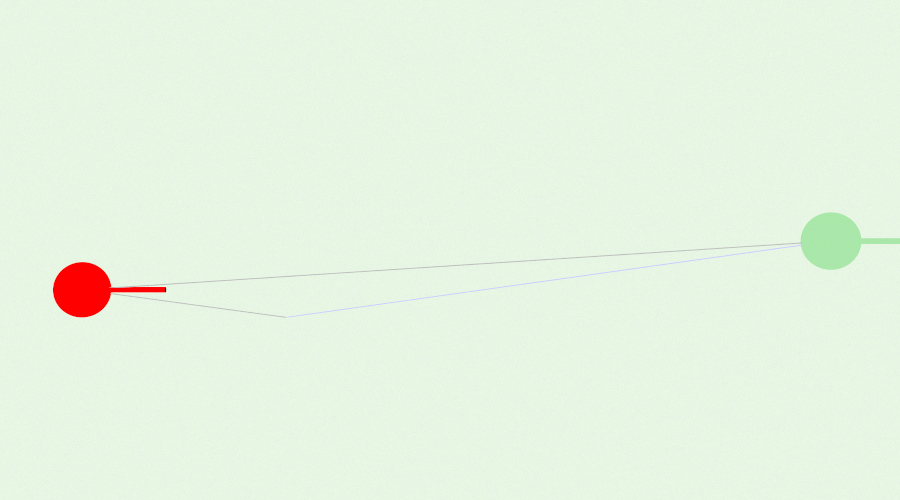
\includegraphics[width=\textwidth,height=0.72\textheight,keepaspectratio]{figures/scene_los.png}
  \end{center}
  \footnotesize Line-of-sight: the direct ray and the ground bounce reach the target.
\end{frame}

\begin{frame}{Render the scenes, with the traced rays}
  \begin{center}
  
\includegraphics[width=\textwidth,height=0.72\textheight,keepaspectratio]{figures/scene_blocked.png}
  \end{center}
  \footnotesize Blocked: the solver finds no path at all -- there are no rays to draw.
\end{frame}

\begin{frame}{Render the scenes, with the traced rays}
  \begin{center}
  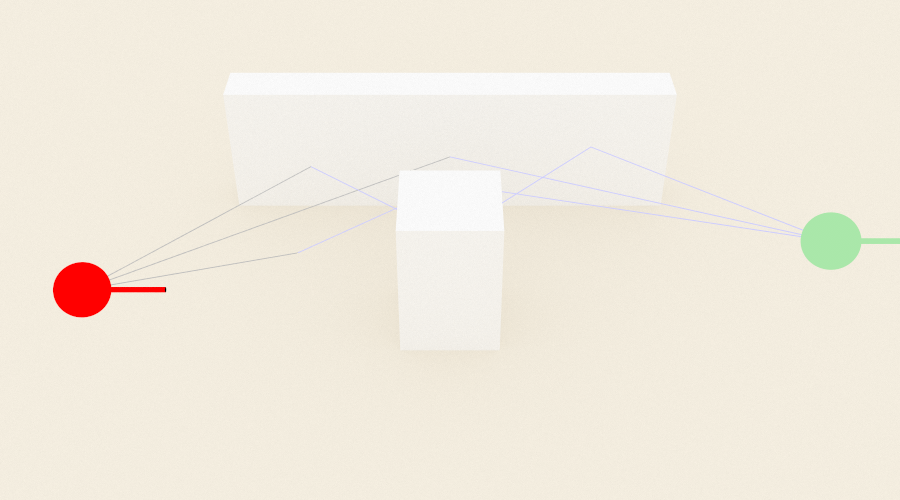
\includegraphics[width=\textwidth,height=0.72\textheight,keepaspectratio]{figures/scene_reflector.png}
  \end{center}
  \footnotesize Blocked + reflector: the wall of the building row mirrors the signal around the blocker (three paths, all longer than the straight line).
\end{frame}

\begin{frame}{The range profiles, side by side}
  One noisy trial per scenario, matched filter output
  against range. Line-of-sight: one clean peak at the true
  301\,m. Blocked: noise, nothing to find. Blocked +
  reflector: a real peak -- but at the detour's length, not
  the target's range. The echo survives the blockage and
  the detection is genuine; the \emph{range} is a lie
  (about $+40$\,m here). A single station cannot tell a
  detour from a distance; resolving that ambiguity takes
  more geometry -- stations that look from somewhere else.
\end{frame}

\begin{frame}[fragile]{The range profiles, side by side --- type this (1/2)}
\begin{lstlisting}[basicstyle=\ttfamily\tiny]
def range_profile_figure(params: BaseStationParams,
                         out_dir="figures"):
    import matplotlib
    matplotlib.use("Agg")
    import matplotlib.pyplot as plt

    os.makedirs(out_dir, exist_ok=True)
    ts = params.sample_period_s
    burst = make_ofdm_burst(params)
    sigma = math.sqrt(params.noise_power_w / 2.0)
    true_range = math.sqrt(300.0**2 + 25.0**2)
    fig, axes = plt.subplots(3, 1, figsize=(7, 7), sharex=True)
    for axis, scenario in zip(axes,
                              ("los", "blocked", "reflector")):
        rt, scene = monostatic_scene(params, scenario)
        _, gains, delays = monostatic_legs(rt, scene)
        total = burst.size + 4096
        echo = np.zeros(total, complex)
        amp_gain = 10.0 ** (params.antenna_gain_dbi / 20.0)
        rcs_factor = math.sqrt(4.0 * math.pi) / params.wavelength_m
        for p in range(gains.size):
            for q in range(gains.size):
                amplitude = (math.sqrt(params.tx_power_w)
                             * amp_gain**2 * gains[p] * gains[q]
                             * rcs_factor)
                echo += amplitude * fractional_delay(
                    burst, (delays[p] + delays[q]) / ts, total)
        rx = echo + sigma * (rng.standard_normal(total)
                             + 1j * rng.standard_normal(total))
        mf = np.abs(np.correlate(rx, burst, mode="valid")) ** 2
\end{lstlisting}
\end{frame}

\begin{frame}[fragile]{The range profiles, side by side --- type this (2/2)}
\begin{lstlisting}[basicstyle=\ttfamily\tiny]
        ranges = (np.arange(mf.size) * ts * SPEED_OF_LIGHT / 2.0)
        keep = ranges <= 600.0
        axis.plot(ranges[keep],
                  10.0 * np.log10(mf[keep] / np.max(mf)))
        axis.axvline(true_range, color="C3", linewidth=0.8)
        axis.set_ylabel(f"{scenario}\n(dB)")
    axes[-1].set_xlabel("range (m)")
    fig.tight_layout()
    fig.savefig(os.path.join(out_dir, "range_profiles.png"),
                dpi=150)
\end{lstlisting}
\end{frame}

\begin{frame}{The range profiles, side by side}
  \begin{center}
  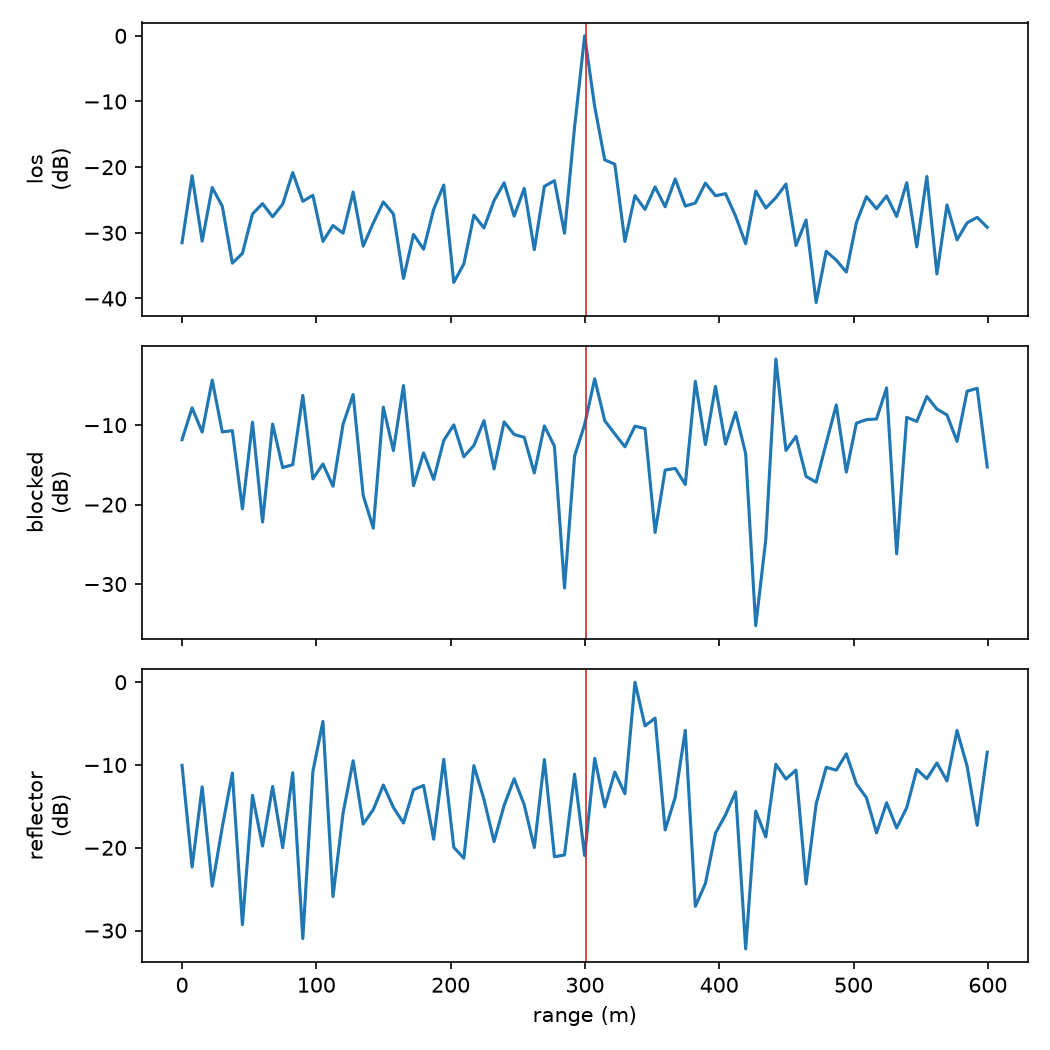
\includegraphics[width=\textwidth,height=0.72\textheight,keepaspectratio]{figures/range_profiles.png}
  \end{center}
  \footnotesize Matched-filter range profiles, one noisy trial per scenario; the vertical line is the true range.
\end{frame}

\begin{frame}{OFDM versus a single tone}
  Same duration, same power, two waveforms. The
  \textbf{OFDM burst} spreads energy over the whole 20\,MHz;
  the \textbf{single tone} concentrates it at one
  frequency. For \emph{frequency and phase} the tone is
  fine -- fit a phase ramp. For \emph{range} the tone is
  nearly blind: range lives in \emph{delay}, delay
  precision comes from \emph{bandwidth} ($c/2B = 7.5$\,m at
  20\,MHz), and the carrier itself carries none. What
  little timing a real tone burst has lives in its slow
  power envelope -- which is why the tone here gets a
  smooth ramp: a rectangular edge would smuggle wideband
  timing into a ``narrowband'' waveform. This is the
  cleanest statement of why sensing wants wideband
  waveforms while synchronization alone can live on a
  tone.
\end{frame}

\begin{frame}[fragile]{OFDM versus a single tone --- type this (1/2)}
\begin{lstlisting}[basicstyle=\ttfamily\tiny]
def make_ofdm_burst(params: BaseStationParams, symbols=20, seed=3):
    burst_rng = np.random.default_rng(seed)
    angles = (burst_rng.integers(0, 4,
                                 (symbols, params.subcarriers))
              * (np.pi / 2.0) + np.pi / 4.0)
    time_symbols = np.fft.ifft(np.exp(1j * angles), axis=1) \
        * math.sqrt(params.subcarriers)
    with_cp = np.concatenate(
        [time_symbols[:, -params.cyclic_prefix:], time_symbols],
        axis=1).reshape(-1)
    return with_cp / math.sqrt(np.mean(np.abs(with_cp) ** 2))


def compare_waveforms(params: BaseStationParams, trials=300,
                      snr_db=10.0, cfo_hz=5e3):
    ts = params.sample_period_s
    ofdm = make_ofdm_burst(params)
    # A single tone at one subcarrier frequency. A real transmitter
    # ramps power smoothly, so the tone gets a smooth (Hann)
    # envelope -- a rectangular edge would smuggle wideband timing
    # information into a "narrowband" waveform.
    tone = (np.exp(2j * np.pi * 3.125e6
                   * np.arange(ofdm.size) * ts)
            * np.hanning(ofdm.size))
    tone = tone / math.sqrt(np.mean(np.abs(tone) ** 2))
    snr = 10.0 ** (snr_db / 10.0)
    sigma = math.sqrt(1.0 / (2.0 * snr))
    results = {}
    for name, burst in (("ofdm", ofdm), ("tone", tone)):
        cfo_errs, delay_errs = [], []
\end{lstlisting}
\end{frame}

\begin{frame}[fragile]{OFDM versus a single tone --- type this (2/2)}
\begin{lstlisting}[basicstyle=\ttfamily\tiny]
        for _ in range(trials):
            delay = int(rng.integers(0, 200))
            rx = fractional_delay(burst, delay, burst.size + 512)
            rx = rx * np.exp(2j * np.pi * cfo_hz
                             * np.arange(rx.size) * ts)
            rx = rx + sigma * (rng.standard_normal(rx.size)
                               + 1j * rng.standard_normal(rx.size))
            # frequency: split-correlation, identical for both
            half = burst.size // 2
            seg = rx[delay : delay + burst.size]
            r = np.sum(np.conj(burst[:half] * seg[half:half+half])
                       * (burst[half:half+half] * np.conj(seg[:half])))
            est = -np.angle(r) / (half * ts) / (2.0 * np.pi)
            cfo_errs.append(est - cfo_hz)
            # delay: matched filter, no help given
            mf = np.abs(np.correlate(rx, burst, mode="valid"))
            delay_errs.append(int(np.argmax(mf)) - delay)
        results[name] = (np.std(cfo_errs),
                         np.sqrt(np.mean(np.square(delay_errs))))
    for name, (cfo_rms, delay_rms) in results.items():
        print(f"  {name:5s} cfo rms {cfo_rms:8.1f} Hz | "
              f"delay rms {delay_rms:8.1f} samples "
              f"({delay_rms * ts * SPEED_OF_LIGHT / 2.0:.0f} m)")
\end{lstlisting}
\end{frame}

\begin{frame}{Localization: from ranges to a position}
  The ghost-range result begs the next step: more stations.
  Four base stations at the corners of the area each run
  the monostatic measurement on the same \textbf{drone}
  (radar cross-section 0.03\,m$^2$, hovering at 60\,m).
  Each station's round-trip delay gives one range -- a
  sphere the drone must sit on -- and four spheres pin the
  position. One ray-tracer solve supplies all four legs
  (ground bounce included); the position solver is
  Gauss--Newton: linearize each range around the current
  guess (the gradient of $\|p - s_i\|$ is the unit vector
  from station to drone), solve the little least-squares
  problem, step, repeat.
\end{frame}

\begin{frame}[fragile]{Localization: from ranges to a position --- type this (1/4)}
\begin{lstlisting}[basicstyle=\ttfamily\tiny]
DRONE = np.array([170.0, 90.0, 60.0])
DRONE_RCS_M2 = 0.03
STATIONS = np.array([[0.0, 0.0, 15.0], [300.0, 0.0, 15.0],
                     [0.0, 200.0, 15.0], [300.0, 200.0, 15.0]])


def localization_legs(params: BaseStationParams):
    """One RT solve, four stations -> drone: [(gains, delays)]."""
    import sionna.rt as rt

    scene = rt.load_scene()
    scene.frequency = params.carrier_frequency_hz
    scene.tx_array = rt.PlanarArray(num_rows=1, num_cols=1,
                                    pattern="iso", polarization="V")
    scene.rx_array = scene.tx_array
    handle = tempfile.NamedTemporaryFile("w", suffix=".ply",
                                         delete=False)
    handle.write(_ply_ground(800.0))
    handle.close()
    try:
        scene.edit(add=rt.SceneObject(
            fname=handle.name, name="ground-plane",
            radio_material=rt.RadioMaterial(
                "ground", thickness=10.0,
                relative_permittivity=15.0, conductivity=0.035)))
    finally:
        os.unlink(handle.name)
    for index, station in enumerate(STATIONS):
        scene.add(rt.Transmitter(f"bs-{index}",
                                 position=station.tolist()))
\end{lstlisting}
\end{frame}

\begin{frame}[fragile]{Localization: from ranges to a position --- type this (2/4)}
\begin{lstlisting}[basicstyle=\ttfamily\tiny]
    scene.add(rt.Receiver("drone", position=DRONE.tolist()))
    paths = rt.PathSolver()(scene, max_depth=3, los=True,
                            specular_reflection=True,
                            diffuse_reflection=False,
                            refraction=False)
    a, tau = paths.cir(normalize_delays=False, out_type="numpy")
    legs = []
    for index in range(len(STATIONS)):
        gains = a[0, 0, index, 0, :, 0]
        delays = tau[0, index, :]
        keep = delays >= 0.0          # padded slots carry tau = -1
        legs.append((gains[keep], delays[keep]))
    return legs


def measure_range(params: BaseStationParams, burst,
                  gains, delays, upsample=16):
    """One noisy monostatic range measurement from one station.

    The peak search runs on a 16x frequency-domain upsampled
    cross-correlation: the coarse three-point parabola on the raw
    sample grid leaves a bias worth several times the noise floor,
    and an estimator meant to be compared against the Cramer-Rao
    bound has to earn it.
    """
    ts = params.sample_period_s
    amp_gain = 10.0 ** (params.antenna_gain_dbi / 20.0)
    rcs_factor = (math.sqrt(4.0 * math.pi * DRONE_RCS_M2)
                  / params.wavelength_m)
    total = burst.size + 2048
\end{lstlisting}
\end{frame}

\begin{frame}[fragile]{Localization: from ranges to a position --- type this (3/4)}
\begin{lstlisting}[basicstyle=\ttfamily\tiny]
    echo = np.zeros(total, complex)
    for p in range(gains.size):
        for q in range(gains.size):
            amplitude = (math.sqrt(params.tx_power_w) * amp_gain**2
                         * gains[p] * gains[q] * rcs_factor)
            echo += amplitude * fractional_delay(
                burst, (delays[p] + delays[q]) / ts, total)
    sigma = math.sqrt(params.noise_power_w / 2.0)
    rx = echo + sigma * (rng.standard_normal(total)
                         + 1j * rng.standard_normal(total))
    spectrum = np.fft.fft(rx) * np.conj(np.fft.fft(burst, total))
    padded = np.zeros(total * upsample, complex)
    padded[: total // 2] = spectrum[: total // 2]
    padded[-total // 2 :] = spectrum[-total // 2 :]
    cc = np.abs(np.fft.ifft(padded)) ** 2
    search = cc[: (total - burst.size) * upsample]
    peak = int(np.argmax(search))
    num = cc[peak - 1] - cc[peak + 1]
    den = cc[peak - 1] - 2 * cc[peak] + cc[peak + 1]
    peak = peak + 0.5 * num / den
    return peak / upsample * ts * SPEED_OF_LIGHT / 2.0, echo


def solve_position(ranges, stations, initial):
    """Gauss-Newton: least-squares position from station ranges.
\end{lstlisting}
\end{frame}

\begin{frame}[fragile]{Localization: from ranges to a position --- type this (4/4)}
\begin{lstlisting}[basicstyle=\ttfamily\tiny]
    The initial guess must sit OFF the stations' common plane:
    every look direction's vertical component is zero there, so the
    plane is a stationary point the iteration can never leave --
    found the hard way (the solver returned z = 15 m forever).
    """
    position = initial.copy()
    for _ in range(20):
        vectors = position - stations
        distances = np.linalg.norm(vectors, axis=1)
        jacobian = vectors / distances[:, None]
        residual = ranges - distances
        step, *_ = np.linalg.lstsq(jacobian, residual, rcond=None)
        position = position + step
        if np.linalg.norm(step) < 1e-6:
            break
    return position
\end{lstlisting}
\end{frame}

\begin{frame}{The Cramer-Rao bound}
  How good could ANY unbiased estimator possibly be? That
  is the Cramer--Rao bound, and both layers of it are
  computable from things already in hand. \textbf{Per
  station (delay):} $\mathrm{var}(\hat\tau) \geq 1 / (8
  \pi^2 \beta^2 \cdot E/N_0)$, where $\beta$ is the
  waveform's rms bandwidth and $E/N_0$ the received echo
  energy over the noise density -- bandwidth and energy are
  the only two currencies delay accuracy trades in (the
  single tone fails exactly here: $\beta \approx 0$).
  Monostatic ranging halves the delay error into range:
  $r = c\tau/2$. \textbf{Position:} each station
  contributes information only ALONG its look direction
  $u_i$; the Fisher information matrix is $J = \sum_i u_i
  u_i^T / \sigma_{r_i}^2$ and $J^{-1}$ lower-bounds the
  position covariance. Geometry enters through the $u_i$:
  directions the stations do not span are directions the
  network cannot measure -- watch the vertical axis.
\end{frame}

\begin{frame}[fragile]{The Cramer-Rao bound --- type this}
\begin{lstlisting}[basicstyle=\ttfamily\tiny]
def rms_bandwidth_hz(burst, sample_rate):
    spectrum = np.abs(np.fft.fft(burst)) ** 2
    freq = np.fft.fftfreq(burst.size, 1.0 / sample_rate)
    center = np.sum(freq * spectrum) / np.sum(spectrum)
    return math.sqrt(np.sum((freq - center) ** 2 * spectrum)
                     / np.sum(spectrum))


def range_crb_m(params: BaseStationParams, burst, echo):
    """Per-station range standard-deviation bound (meters)."""
    beta = rms_bandwidth_hz(burst, params.bandwidth_hz)
    # E/N0: echo energy over noise density, in sample units.
    energy_over_n0 = np.sum(np.abs(echo) ** 2) / params.noise_power_w
    var_tau = 1.0 / (8.0 * math.pi**2 * beta**2 * energy_over_n0)
    return (SPEED_OF_LIGHT / 2.0) * math.sqrt(var_tau)


def position_bound(stations, drone, range_sigmas):
    """Cramer-Rao covariance for the position (3x3)."""
    vectors = drone - stations
    units = vectors / np.linalg.norm(vectors, axis=1)[:, None]
    fisher = np.zeros((3, 3))
    for u, sigma in zip(units, range_sigmas):
        fisher += np.outer(u, u) / sigma**2
    return np.linalg.inv(fisher)
\end{lstlisting}
\end{frame}

\begin{frame}{Localize the drone, and check against the bound}
  200 full trials: four noisy matched-filter ranges, one
  Gauss--Newton solve each; then measured error next to
  the bound, axis by axis. Measured: per-station range
  bound 21\,cm; position \textbf{spread} x/y/z =
  0.16/0.25/0.49\,m against bounds 0.14/0.18/0.43\,m --
  the estimator runs within 20--40\% of the theoretical
  limit on every axis. Two lessons in those numbers.
  \textbf{Geometry}: the vertical bound is 3$\times$ the
  horizontal ones before a single trial runs -- all four
  stations sit below the drone in nearly a plane, so their
  look directions barely span the vertical. \textbf{Bias
  is not spread}: on top of the spread sits a systematic
  error (x $-0.34$, y $+0.24$, z $+3.4$\,m) from the
  ground-bounce path fusing with the direct one inside the
  resolution cell. The bound only governs an unbiased
  estimator's spread; multipath is a modeling error, it
  does not average away, and the weak axis amplifies it --
  the same lesson as the ghost target, in miniature.
\end{frame}

\begin{frame}[fragile]{Localize the drone, and check against the bound --- type this (1/2)}
\begin{lstlisting}[basicstyle=\ttfamily\tiny]
def localization_study(params: BaseStationParams, trials=200,
                       out_dir="figures"):
    import matplotlib
    matplotlib.use("Agg")
    import matplotlib.pyplot as plt

    burst = make_ofdm_burst(params)
    legs = localization_legs(params)
    initial = np.array([150.0, 100.0, 120.0])  # off the plane!

    # Per-station bounds from one clean echo each.
    sigmas = []
    for gains, delays in legs:
        _, echo = measure_range(params, burst, gains, delays)
        sigmas.append(range_crb_m(params, burst, echo))
    bound = position_bound(STATIONS, DRONE, sigmas)

    estimates = []
    for _ in range(trials):
        ranges = np.array([
            measure_range(params, burst, gains, delays)[0]
            for gains, delays in legs])
        estimates.append(solve_position(ranges, STATIONS, initial))
    estimates = np.array(estimates)
    errors = estimates - DRONE
\end{lstlisting}
\end{frame}

\begin{frame}[fragile]{Localize the drone, and check against the bound --- type this (2/2)}
\begin{lstlisting}[basicstyle=\ttfamily\tiny]
    print("localization of the drone (200 trials, 4 stations):")
    print(f"  per-station range bound : "
          f"{np.mean(sigmas)*100:.1f} cm")
    # The bound limits the SPREAD of an unbiased estimator; the
    # multipath bias is a separate, systematic effect -- report both.
    for axis, name in enumerate("xyz"):
        print(f"  {name}: bias {np.mean(errors[:, axis]):+7.3f} m"
              f"  spread {np.std(errors[:, axis]):6.3f} m"
              f"  | bound {math.sqrt(bound[axis, axis]):6.3f} m")

    # Scatter in the horizontal plane with the 3-sigma ellipse.
    os.makedirs(out_dir, exist_ok=True)
    fig, axis = plt.subplots(figsize=(6, 5))
    axis.scatter(estimates[:, 0], estimates[:, 1], s=6)
    values, directions = np.linalg.eigh(bound[:2, :2])
    angle = np.linspace(0.0, 2.0 * np.pi, 200)
    circle = np.stack([np.cos(angle), np.sin(angle)])
    ellipse = (directions
               @ np.diag(3.0 * np.sqrt(values)) @ circle)
    axis.plot(DRONE[0] + ellipse[0], DRONE[1] + ellipse[1], "C3")
    axis.plot(DRONE[0], DRONE[1], "k+")
    axis.set_xlabel("x (m)")
    axis.set_ylabel("y (m)")
    axis.set_aspect("equal")
    fig.tight_layout()
    fig.savefig(os.path.join(out_dir, "localization_scatter.png"),
                dpi=150)
    return sigmas, bound, errors
\end{lstlisting}
\end{frame}

\begin{frame}{Localize the drone, and check against the bound}
  \begin{center}
  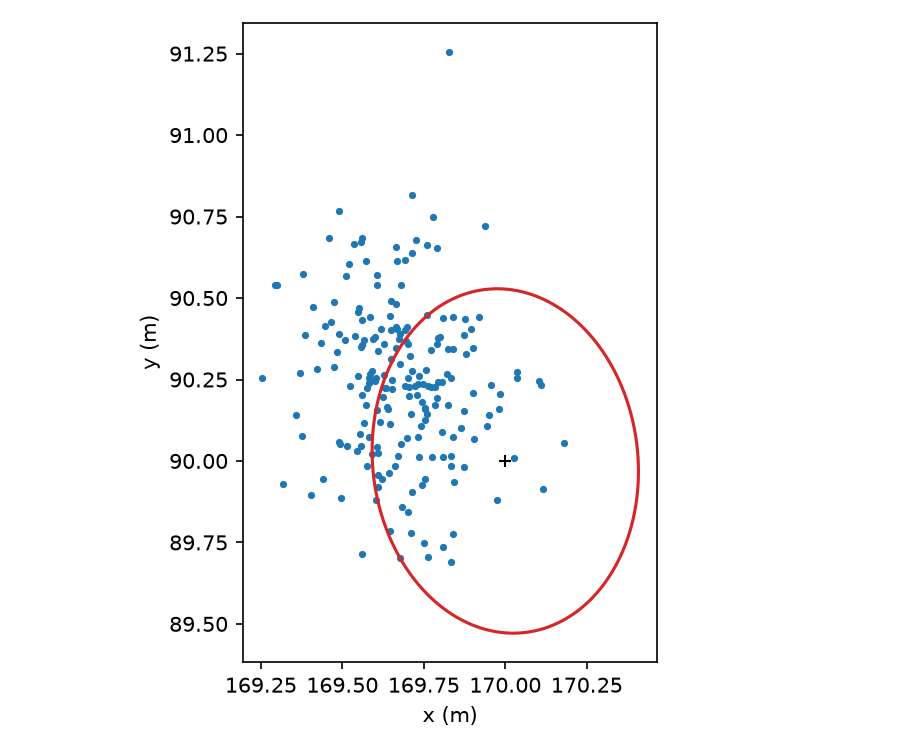
\includegraphics[width=\textwidth,height=0.72\textheight,keepaspectratio]{figures/localization_scatter.png}
  \end{center}
  \footnotesize 200 position estimates (horizontal plane), the true position (+), and the bound's 3-sigma ellipse. The cloud's SIZE matches the ellipse -- the spread is near the bound -- but the cloud sits displaced from the truth: that offset is the multipath bias, and no amount of averaging shrinks it.
\end{frame}

\begin{frame}{Ghosts: put the target IN the scene}
  Everything so far modeled the target as a point probe
  plus an analytic radar cross-section. That is the right
  tool for a link budget, and it is wrong for this
  question, because it can only ever return the target.
  A sensing receiver does not get a clean target return --
  it gets everything in the scene that sends energy back,
  and the hard part of the job is that most of those
  returns are not the object. So here the target becomes
  \textbf{geometry}: a $4{\times}2{\times}1.5$\,m metal
  box at the target position, meshed into the scene like
  any building. Each station gets a receiver co-located
  with its transmitter, and the solver is asked for the
  round trips directly -- station\,$\to$\,anything\,$\to$
  \,same station. No radar cross-section is applied and no
  legs are paired by hand: whatever comes back, comes back.
\end{frame}

\begin{frame}[fragile]{Ghosts: put the target IN the scene --- type this (1/2)}
\begin{lstlisting}[basicstyle=\ttfamily\tiny]
TARGET_BOX = (4.0, 2.0, 1.5)          # w, d, h -- vehicle class
GHOST_BLOCKER = (250.0, 160.0, 36.0, 36.0, 60.0)   # x, y, w, d, h
GHOST_WALL = (150.0, 250.0, 400.0, 10.0, 60.0)
LEAKAGE_GATE_M = 30.0   # ignore returns closer than this


def multipath_scene(params: BaseStationParams, scenario: str,
                    with_target=True):
    """Four stations + a MESHED target in a built-up scene.

    with_target=False builds the identical scene minus the target --
    that is the clutter reference the study subtracts.
    """
    import sionna.rt as rt

    scene = rt.load_scene()
    scene.frequency = params.carrier_frequency_hz
    scene.tx_array = rt.PlanarArray(num_rows=1, num_cols=1,
                                    pattern="iso", polarization="V")
    scene.rx_array = scene.tx_array
    ground, concrete = _materials(rt)
    _add_mesh(rt, scene, "ground-plane", _ply_ground(800.0), ground)
    if scenario in ("multipath", "nlos"):
        _add_mesh(rt, scene, "building-row",
                  _ply_box(*GHOST_WALL), concrete)
    if scenario == "nlos":
        _add_mesh(rt, scene, "blocker",
                  _ply_box(*GHOST_BLOCKER), concrete)
\end{lstlisting}
\end{frame}

\begin{frame}[fragile]{Ghosts: put the target IN the scene --- type this (2/2)}
\begin{lstlisting}[basicstyle=\ttfamily\tiny]
    # The target itself, as an object. Metal: a conductor reflects
    # essentially everything, which is the point -- this is the one
    # thing in the scene we WANT to come back.
    if with_target:
        metal = rt.RadioMaterial("target-metal", thickness=0.002,
                                 relative_permittivity=1.0,
                                 conductivity=1e7,
                                 color=(0.85, 0.10, 0.10))
        width, depth, height = TARGET_BOX
        _add_mesh(rt, scene, "target",
                  _ply_box(DRONE[0], DRONE[1], width, depth, height,
                           z0=DRONE[2] - height / 2.0), metal)

    # Monostatic means the receiver IS the transmitter, so every
    # station gets both. They are separated by half a meter rather
    # than placed on the same point: a zero-length transmitter-to-
    # receiver path is a degenerate case for a path solver, and at
    # 200 m range half a meter changes no delay that matters (it is
    # 1/15th of a resolution cell).
    for index, station in enumerate(STATIONS):
        scene.add(rt.Transmitter(f"bs-{index}",
                                 position=station.tolist()))
        receiver = station + np.array([0.0, 0.0, 0.5])
        scene.add(rt.Receiver(f"rx-{index}",
                              position=receiver.tolist()))
    return rt, scene
\end{lstlisting}
\end{frame}

\begin{frame}{What actually comes back}
  One solve gives every station its own round trips. Two
  pieces of bookkeeping. \textbf{Leakage}: a receiver
  sitting on its own transmitter sees a zero-length path
  -- in hardware this is the coupling that saturates the
  front end, and in both cases it is gated out by range.
  \textbf{Everything else is a return, and the solver does
  not label them.} Nothing in the output says ``this one
  is the target.'' The station gets the target echo, the
  ground under its own feet, the wall of the building row
  245\,m away, the target-then-wall double bounce -- all
  as one list of (gain, delay) pairs, exactly as a real
  receiver gets them summed into one waveform.
\end{frame}

\begin{frame}[fragile]{What actually comes back --- type this (1/2)}
\begin{lstlisting}[basicstyle=\ttfamily\tiny]
def monostatic_returns(rt, scene, min_range_m=LEAKAGE_GATE_M):
    """One solve -> [(gains, delays)] of round trips per station."""
    paths = rt.PathSolver()(scene, max_depth=3, los=True,
                            specular_reflection=True,
                            diffuse_reflection=False,
                            refraction=False)
    a, tau = paths.cir(normalize_delays=False, out_type="numpy")
    # a: [rx, rx_ant, tx, tx_ant, path, time]; tau: [rx, tx, path].
    # Monostatic = the diagonal: station i transmitting, station i
    # listening. The off-diagonal entries are the bistatic pairs --
    # real, useful, and a bigger study than this one.
    minimum_delay = 2.0 * min_range_m / SPEED_OF_LIGHT
    returns = []
    for index in range(len(STATIONS)):
        gains = a[index, 0, index, 0, :, 0]
        delays = tau[index, index, :]
        keep = delays >= minimum_delay      # drops padding AND leakage
        returns.append((gains[keep], delays[keep]))
    return paths, returns


def roundtrip_echo(params: BaseStationParams, burst, gains, delays,
                   pad=4096):
    """Sum the traced round trips into one received waveform.
\end{lstlisting}
\end{frame}

\begin{frame}[fragile]{What actually comes back --- type this (2/2)}
\begin{lstlisting}[basicstyle=\ttfamily\tiny]
    Contrast this with the probe model earlier: there, one-way legs
    had to be paired (p out, q back) and a radar cross-section
    supplied by hand. Here each entry already IS a round trip, so
    the echo is a plain sum -- and it contains the clutter too.
    """
    ts = params.sample_period_s
    amp_gain = 10.0 ** (params.antenna_gain_dbi / 20.0)
    total = burst.size + pad
    echo = np.zeros(total, complex)
    for p in range(gains.size):
        amplitude = (math.sqrt(params.tx_power_w) * amp_gain**2
                     * gains[p])
        echo += amplitude * fractional_delay(
            burst, delays[p] / ts, total)
    return echo
\end{lstlisting}
\end{frame}

\begin{frame}{Every peak is a candidate range}
  The matched filter now returns a \emph{comb}, and the
  detector has no way to know which peak is the target --
  so take them all. The obvious way to peel them off is to
  find the largest, blank a resolution cell around it, and
  repeat; do that and the detector immediately reports
  three targets where there is one, because a burst's
  autocorrelation has \textbf{sidelobes} and the first
  pair sits about 2.5 cells out -- outside the blanked
  window and far above the noise floor. Sidelobes are not
  noise; they are a known, deterministic feature of the
  waveform, so they can be removed exactly. That is
  \textbf{CLEAN}: each time a peak is accepted, subtract a
  correctly scaled and shifted copy of the burst's own
  autocorrelation -- the full shape a single return makes,
  sidelobes included -- and look again at what is left.
  The correlation is also upsampled 16$\times$, for the
  reason \texttt{measure\_range} gives: the coarse
  parabola biases a peak by meters, and the residual test
  below cannot tell a wrong association from a biased
  right one if the right one is already off by half a cell.
\end{frame}

\begin{frame}[fragile]{Every peak is a candidate range --- type this (1/2)}
\begin{lstlisting}[basicstyle=\ttfamily\tiny]
def _upsampled(spectrum, total, upsample):
    padded = np.zeros(total * upsample, complex)
    padded[: total // 2] = spectrum[: total // 2]
    padded[-total // 2:] = spectrum[-total // 2:]
    return np.fft.ifft(padded)


def range_peaks(params: BaseStationParams, burst, echo,
                max_peaks=4, upsample=16, snr_gate=30.0):
    """All candidate ranges in one echo; (ranges_m, profile, grid)."""
    ts = params.sample_period_s
    if echo.size == 0:
        return np.zeros(0), np.zeros(0), np.zeros(0)
    total = echo.size
    sigma = math.sqrt(params.noise_power_w / 2.0)
    rx = echo + sigma * (rng.standard_normal(total)
                         + 1j * rng.standard_normal(total))
    burst_spectrum = np.fft.fft(burst, total)
    correlation = _upsampled(np.fft.fft(rx) * np.conj(burst_spectrum),
                             total, upsample)
    # The response a SINGLE return produces: the burst correlated
    # with itself, at the same upsampling. This is what CLEAN
    # subtracts, and why sidelobes come out with the peak.
    template = _upsampled(np.abs(burst_spectrum) ** 2, total,
                          upsample)
    search = (total - burst.size) * upsample
    profile = np.abs(correlation[:search]) ** 2
    grid = (np.arange(search) / upsample * ts
            * SPEED_OF_LIGHT / 2.0)
\end{lstlisting}
\end{frame}

\begin{frame}[fragile]{Every peak is a candidate range --- type this (2/2)}
\begin{lstlisting}[basicstyle=\ttfamily\tiny]
    floor = np.median(profile)
    ranges = []
    while len(ranges) < max_peaks:
        power = np.abs(correlation[:search]) ** 2
        index = int(np.argmax(power))
        if power[index] < snr_gate * floor:
            break
        refined = float(index)
        if 0 < index < search - 1:
            num = power[index - 1] - power[index + 1]
            den = (power[index - 1] - 2 * power[index]
                   + power[index + 1])
            if den != 0.0:
                refined = index + 0.5 * num / den
        ranges.append(refined / upsample * ts * SPEED_OF_LIGHT / 2.0)
        amplitude = correlation[index] / template[0]
        correlation = correlation - amplitude * np.roll(template,
                                                        index)
    return np.array(sorted(ranges)), profile, grid
\end{lstlisting}
\end{frame}

\begin{frame}{Association: where the ghosts come from}
  Now the network has to decide which peak at station $i$
  belongs to the same object as which peak at station $j$
  -- the \textbf{association} problem, and it is
  combinatorial: with four candidates at each of four
  stations there are $4^4 = 256$ ways to pick one range
  each, and 255 of them are wrong. Each combination is a
  perfectly well-posed least-squares problem returning a
  perfectly plausible position. Those are the
  \textbf{ghost targets}. What saves the network is that
  four ranges determine three coordinates, leaving one
  degree of freedom: a wrong combination generally cannot
  be fitted by ANY position, so its residual is large and
  it can be gated away. Note the corollary, which is the
  real argument for the fourth station: with three
  stations the fit is exact, the residual is identically
  zero, and \emph{no} ghost can ever be rejected.
\end{frame}

\begin{frame}[fragile]{Association: where the ghosts come from --- type this}
\begin{lstlisting}[basicstyle=\ttfamily\tiny]
def associate(candidates, stations, initial):
    """Every one-peak-per-station combination -> a fix.

    Returns [(position, residual_rms_m)], one per combination.
    """
    fixes = []
    for combination in itertools.product(*candidates):
        ranges = np.array(combination)
        position = solve_position(ranges, stations, initial)
        if not np.all(np.isfinite(position)):
            continue
        residual = ranges - np.linalg.norm(position - stations,
                                           axis=1)
        fixes.append((position,
                      float(np.sqrt(np.mean(residual**2)))))
    return fixes
\end{lstlisting}
\end{frame}

\begin{frame}{Clutter cancellation, and what it cannot remove}
  Run the scene as built and the target is invisible --
  not marginal, invisible. A building wall reflects
  \emph{specularly}, so its return behaves like a mirror
  image of the transmitter and falls off as one-way
  spreading over the folded path; the target's return is a
  radar return and falls off as $r^{-4}$. The wall wins by
  tens of dB, and every peak the detector reports is the
  building. This is the real first problem in sensing, and
  it has a standard answer: the clutter does not move.
  Solve the identical scene \emph{without} the target,
  subtract that echo, and the static returns cancel. (In
  hardware the same cancellation is done in Doppler --
  same idea, and the reference is measured rather than
  simulated.) Now the important part: what survives the
  subtraction is everything that \emph{touched} the
  target, and that includes station\,$\to$\,target\,$\to$
  \,wall\,$\to$\,station. Clutter cancellation removes the
  scene; it cannot remove the target's own multipath. The
  ghosts come from what is left.
\end{frame}

\begin{frame}{The ghost study, and the picture of it}
  One run per scenario: solve the scene twice (with and
  without the target), cancel, pull every peak, enumerate
  the associations, gate on the residual, report what
  survives. Read the map as three claims. \texttt{open}:
  nothing but ground and target, association is nearly
  unique. \texttt{multipath}: the target is also seen
  around the building row, so each station reports extra
  ranges and a lattice of ghost fixes appears; the
  residual gate kills most, and the survivors are the
  dangerous ones -- consistent positions where nothing is
  flying. \texttt{nlos}: the blocker removes the north-east
  station's direct view, so its only target-bearing return
  is the detour and the best association is confidently
  wrong. That is the failure worth remembering: not a
  large error announcing itself, but a small residual on
  the wrong answer.
\end{frame}

\begin{frame}[fragile]{The ghost study, and the picture of it --- type this (1/5)}
\begin{lstlisting}[basicstyle=\ttfamily\tiny]
def ghost_study(params: BaseStationParams, gate_m=2.0,
                out_dir="figures"):
    import matplotlib
    matplotlib.use("Agg")
    import matplotlib.pyplot as plt

    os.makedirs(out_dir, exist_ok=True)
    burst = make_ofdm_burst(params)
    initial = np.array([150.0, 100.0, 120.0])   # off the plane!
    true_ranges = np.linalg.norm(DRONE - STATIONS, axis=1)
    scenarios = ("open", "multipath", "nlos")
    fig_map, map_axes = plt.subplots(1, 3, figsize=(13, 4.6),
                                     sharex=True, sharey=True)
    fig_pro, pro_axes = plt.subplots(len(STATIONS), 3,
                                     figsize=(13, 8), sharex=True)
    for column, scenario in enumerate(scenarios):
        rt, scene = multipath_scene(params, scenario)
        _, returns = monostatic_returns(rt, scene)
        rt, empty_scene = multipath_scene(params, scenario,
                                          with_target=False)
        _, clutter = monostatic_returns(rt, empty_scene)
        candidates, profiles, grids, raw_profiles = [], [], [], []
        for (gains, delays), (cg, cd) in zip(returns, clutter):
            echo = roundtrip_echo(params, burst, gains, delays)
            reference = roundtrip_echo(params, burst, cg, cd)
            # Noise is added once, inside range_peaks: the reference
            # is a stored clutter map, not a second noisy capture.
            ranges, profile, grid = range_peaks(params, burst,
                                                echo - reference)
            candidates.append(ranges)
\end{lstlisting}
\end{frame}

\begin{frame}[fragile]{The ghost study, and the picture of it --- type this (2/5)}
\begin{lstlisting}[basicstyle=\ttfamily\tiny]
            profiles.append(profile)
            grids.append(grid)
            raw_profiles.append(range_peaks(params, burst, echo)[1])

        # Did the ray tracer actually find the target? A peak within
        # one resolution cell of the true range says yes. This is
        # the check that decides whether the run means anything.
        cell = SPEED_OF_LIGHT / (2.0 * params.bandwidth_hz)
        found = [bool(np.any(np.abs(c - t) < cell))
                 for c, t in zip(candidates, true_ranges)]
        counts = [len(c) for c in candidates]
        print(f"  {scenario:9s}: returns/station "
              f"{[g.size for g, _ in returns]}, peaks {counts}, "
              f"target seen by {sum(found)}/{len(found)} stations")

        if min(counts) == 0:
            fixes, kept = [], []
            print("             a station heard nothing at all -- "
                  "no fix is possible")
        else:
            fixes = associate(candidates, STATIONS, initial)
            kept = [f for f in fixes if f[1] <= gate_m]
            print(f"             {len(fixes)} associations, "
                  f"{len(kept)} survive the {gate_m:.0f} m gate")
        if kept:
            errors = [np.linalg.norm(p - DRONE) for p, _ in kept]
            best = min(kept, key=lambda f: f[1])
            # Two separate questions, and they have different
            # answers: is the truth still in the surviving set, and
            # does the survivor the network would PICK happen to be
\end{lstlisting}
\end{frame}

\begin{frame}[fragile]{The ghost study, and the picture of it --- type this (3/5)}
\begin{lstlisting}[basicstyle=\ttfamily\tiny]
            # it? A ghost can fit better than the target.
            truth_survives = min(errors) < 5.0
            print(f"             {sum(e > 5.0 for e in errors)} of "
                  f"{len(kept)} survivors are ghosts; truth "
                  f"{'survives' if truth_survives else 'is GONE'} "
                  f"(closest {min(errors):.1f} m)")
            print(f"             lowest-residual fix is "
                  f"{np.linalg.norm(best[0] - DRONE):6.1f} m from "
                  f"the target (residual {best[1]:.2f} m)")

        axis = map_axes[column]
        buildings = []
        if scenario in ("multipath", "nlos"):
            buildings.append(GHOST_WALL)
        if scenario == "nlos":
            buildings.append(GHOST_BLOCKER)
        for bx, by, bw, bd, _ in buildings:
            axis.add_patch(plt.Rectangle((bx - bw / 2, by - bd / 2),
                                         bw, bd, color="0.75"))
        rejected = np.array([p for p, r in fixes if r > gate_m])
        survived = np.array([p for p, r in kept])
        if rejected.size:
            axis.scatter(rejected[:, 0], rejected[:, 1], s=18,
                         facecolors="none", edgecolors="0.6",
                         label="rejected by residual")
        if survived.size:
            axis.scatter(survived[:, 0], survived[:, 1], s=26,
                         color="C3", label="survives the gate")
        axis.scatter(STATIONS[:, 0], STATIONS[:, 1], marker="s",
                     s=45, color="C0", label="base stations")
\end{lstlisting}
\end{frame}

\begin{frame}[fragile]{The ghost study, and the picture of it --- type this (4/5)}
\begin{lstlisting}[basicstyle=\ttfamily\tiny]
        axis.plot(DRONE[0], DRONE[1], "k+", markersize=14,
                  markeredgewidth=2, label="true target")
        axis.set_title(scenario)
        axis.set_xlabel("x (m)")
        axis.set_aspect("equal")
        if column == 0:
            axis.set_ylabel("y (m)")
            axis.legend(fontsize=7, loc="upper left")

        for row in range(len(STATIONS)):
            paxis = pro_axes[row, column]
            profile, grid = profiles[row], grids[row]
            if profile.size:
                keep = grid <= 500.0
                paxis.semilogy(grid[keep], raw_profiles[row][keep],
                               lw=0.7, color="0.7",
                               label="before cancellation")
                paxis.semilogy(grid[keep], profile[keep], lw=0.8,
                               color="C0", label="after")
                for candidate in candidates[row]:
                    paxis.axvline(candidate, color="C3", lw=0.8,
                                  ls=":")
            paxis.axvline(true_ranges[row], color="k", lw=1.0)
            if row == 0 and column == 0:
                paxis.legend(fontsize=6)
            if column == 0:
                paxis.set_ylabel(f"bs-{row}")
            if row == 0:
                paxis.set_title(scenario)
            if row == len(STATIONS) - 1:
\end{lstlisting}
\end{frame}

\begin{frame}[fragile]{The ghost study, and the picture of it --- type this (5/5)}
\begin{lstlisting}[basicstyle=\ttfamily\tiny]
                paxis.set_xlabel("range (m)")

    fig_map.tight_layout()
    fig_map.savefig(os.path.join(out_dir, "ghost_map.png"), dpi=150)
    fig_pro.tight_layout()
    fig_pro.savefig(os.path.join(out_dir, "ghost_profiles.png"),
                    dpi=150)


def render_ghost_scene(params: BaseStationParams,
                       out_dir="figures"):
    os.makedirs(out_dir, exist_ok=True)
    rt, scene = multipath_scene(params, "nlos")
    paths, _ = monostatic_returns(rt, scene)      # SOLVE FIRST
    add_visual_markers(rt, scene, STATIONS, DRONE, scale=16.0)
    camera = rt.Camera(position=[150.0, -430.0, 420.0],
                       look_at=[150.0, 120.0, 30.0])
    scene.render_to_file(
        camera=camera,
        filename=os.path.join(out_dir, "scene_ghost.png"),
        paths=paths, show_devices=False, resolution=(900, 560))
\end{lstlisting}
\end{frame}

\begin{frame}{The ghost study, and the picture of it}
  \begin{center}
  \includegraphics[width=\textwidth,height=0.72\textheight,keepaspectratio]{figures/ghost_profiles.png}
  \end{center}
  \footnotesize Matched-filter range profiles, one row per station, one column per scenario. Solid line = the target's true range; dotted lines = the peaks the detector actually reports. Every peak that is not on the solid line is a return from something that is not the target.
\end{frame}

\begin{frame}{The ghost study, and the picture of it}
  \begin{center}
  \includegraphics[width=\textwidth,height=0.72\textheight,keepaspectratio]{figures/ghost_map.png}
  \end{center}
  \footnotesize Every association, solved. Hollow circles are combinations the residual gate rejects; filled circles survive. Open ground gives essentially one answer; the building row breeds a lattice of ghosts and some are consistent enough to survive; under blockage the surviving cluster no longer contains the truth.
\end{frame}

\begin{frame}{The ghost study, and the picture of it}
  \begin{center}
  \includegraphics[width=\textwidth,height=0.72\textheight,keepaspectratio]{figures/scene_ghost.png}
  \end{center}
  \footnotesize The NLOS scene as the ray tracer sees it, with every traced round trip drawn: the blocker cutting the north-east station off, and the building row returning the detour that replaces it. The target IS in this scene as a 4 m metal box -- the enlarged red marker around it is drawn after the solve, so the picture can show where it is.
\end{frame}

\begin{frame}{Run Part II}
  Everything measured in one run (exact output below the
  code). Training fields: 500/500 exact timing, 1.03\,kHz
  frequency error, 0.107\,rad phase spread. Monostatic
  sensing, line-of-sight: 2 paths (direct + ground bounce),
  echo $-97.5$\,dBm -- below the $-94$\,dBm floor, saved by
  the matched filter's 32\,dB -- detection 100\%, range
  error $-1.2 \pm 0.03$\,m (the small bias is the ground
  bounce's slightly longer path pulling the peak). Blocked:
  the solver finds \textbf{zero} paths -- no echo exists at
  all, detection 0\%; at these scales blockage is total,
  not a few dB. Blocked + reflector: the detour restores an
  echo ($-109.2$\,dBm, detection 54\%) but the measured
  range is \textbf{$+37.4 \pm 1.2$\,m wrong} -- a ghost
  target at the detour's length. One station cannot tell a
  detour from a distance: the concrete argument for a
  \emph{distributed} array that looks from several places
  at once. Waveforms at 10\,dB: OFDM delay error 0.0
  samples rms; the smoothed tone 2.8 samples (21\,m), all
  of it from the envelope; frequency: both at the few-kHz
  level set by the 40\,$\mu$s burst duration.
\end{frame}

\begin{frame}[fragile]{Run Part II --- type this (1/2)}
\begin{lstlisting}[basicstyle=\ttfamily\tiny]
if __name__ == "__main__":
    params = BaseStationParams()
    print(f"noise floor: "
          f"{10*math.log10(params.noise_power_w)+30:.1f} dBm")

    print("training fields (500 trials, 15 dB, 20 kHz offset):")
    test_training_fields(params)

    burst = make_ofdm_burst(params)
    for scenario in ("los", "blocked", "reflector"):
        rt, scene = monostatic_scene(params, scenario)
        _, gains, delays = monostatic_legs(rt, scene)
        rate, errors, echo_power = monostatic_range(
            params, burst, gains, delays)
        echo_dbm = (10 * math.log10(echo_power) + 30
                    if echo_power > 0 else float("-inf"))
        line = (f"monostatic {scenario:10s}: {gains.size} paths, "
                f"echo {echo_dbm:6.1f} dBm, "
                f"detection {rate*100:3.0f} %")
        if errors.size:
            line += (f", range error {np.mean(errors):+.1f} "
                     f"+- {np.std(errors):.1f} m")
        print(line)

    print("waveforms (300 trials, 10 dB, 5 kHz offset):")
    compare_waveforms(params)

    localization_study(params)
\end{lstlisting}
\end{frame}

\begin{frame}[fragile]{Run Part II --- type this (2/2)}
\begin{lstlisting}[basicstyle=\ttfamily\tiny]
    print("ghosts (4 stations, built-up scene):")
    ghost_study(params)

    print("rendering scenes and range profiles into figures/ ...")
    render_scenes(params)
    range_profile_figure(params)
    render_ghost_scene(params)
\end{lstlisting}
\end{frame}

\begin{frame}[fragile]{Part II --- measured output}
  The exact output of \texttt{build\_sensing.py} when this
  guide was generated:
\begin{lstlisting}[language={},basicstyle=\ttfamily\tiny]
noise floor: -94.0 dBm
training fields (500 trials, 15 dB, 20 kHz offset):
  timing exact      : 500/500
  cfo error rms     : 1030.2 Hz (0.294 ppm)
  phase spread rms  : 0.1068 rad
monostatic los       : 2 paths, echo  -97.5 dBm,
    detection 100 %, range error -1.2 +- 0.0 m
monostatic blocked   : 0 paths, echo   -inf dBm,
    detection   0 %
monostatic reflector : 3 paths, echo -109.2 dBm,
    detection  54 %, range error +37.4 +- 1.2 m
waveforms (300 trials, 10 dB, 5 kHz offset):
  ofdm  cfo rms   2340.9 Hz | delay rms  0.0 samples (0 m)
  tone  cfo rms   7108.6 Hz | delay rms  2.8 samples (21 m)
localization of the drone (200 trials, 4 stations):
  per-station range bound : 21.2 cm
  x: bias  -0.318 m  spread  0.163 m  | bound  0.136 m
  y: bias  +0.245 m  spread  0.244 m  | bound  0.176 m
  z: bias  +3.441 m  spread  0.507 m  | bound  0.427 m
\end{lstlisting}
\end{frame}


\begin{frame}{Where to go from here}
  \begin{itemize}
    \item \textbf{Break your own builds} (you can, they are your
      files): feed Part I's filter only the forward capture --- it
      locks to the channel phase, confidently wrong. Delete the
      $\pi$ check --- about half of seeds settle at zero gain
      reporting lock. In Part II, replace the tone's smooth ramp
      with a rectangular edge and watch it ``gain'' range accuracy
      it does not deserve.
    \item \textbf{The same code at $N$ stations}:
      \texttt{ota\_sync/network.py} (star), \texttt{microsync.py},
      \texttt{scheduled.py}, \texttt{dfpc.py},
      \texttt{hybrid\_calibration/} --- all built on the classes you
      wrote in Part I.
    \item \textbf{What it leads to}: \texttt{topology\_selection/}
      --- at $N$ stations you choose which pairs exchange and how
      corrections apply, and those choices are not separable. And
      Part II's blocked-echo result is the argument for sensing with
      a \emph{distributed} array in the first place.
    \item Regenerate this guide after any change:
      \texttt{python3 extract\_build.py \&\& python3 gen\_slides.py
      \&\& tectonic phase\_sync\_coding\_guide.tex}
  \end{itemize}
\end{frame}

\end{document}
